\documentclass[../relativity_main.tex]{subfiles}
% \documentclass[ngerman, DIV=11, BCOR=0mm, paper=a4, fontsize=11pt, parskip=half, twoside=false, titlepage=true]{scrreprt}
%\graphicspath{ {Bilder/} {../Bilder/} }


\usepackage[singlespacing]{setspace}
\usepackage{lastpage}
\usepackage[automark, headsepline]{scrlayer-scrpage}
\clearscrheadings
\setlength{\headheight}{\baselineskip}
%\automark[part]{section}
\automark[chapter]{chapter}
\automark*[chapter]{section} %mithilfe des * wird nur ergänzt; bei vorhandener section soll also das in der Kopfzeile stehen
\automark*[chapter]{subsection}
\ihead[]{\headmark}
%\ohead[]{Seite~\thepage}
\cfoot{\hypersetup{linkcolor=black}Seite~\thepage~von~\pageref{LastPage}}

\usepackage[utf8]{inputenc}
\usepackage[ngerman, english]{babel}
\usepackage[expansion=true, protrusion=true]{microtype}
\usepackage{amsmath}
\usepackage{amsfonts}
\usepackage{amsthm}
\usepackage{amssymb}
\usepackage{mathtools}
\usepackage{mathdots}
\usepackage{aligned-overset} % otherwise, overset/underset shift alignment
\usepackage{upgreek}
\usepackage[free-standing-units]{siunitx}
\usepackage{esvect}
\usepackage{graphicx}
\usepackage{epstopdf}
\usepackage[hypcap]{caption}
\usepackage{booktabs}
\usepackage{flafter}
\usepackage[section]{placeins}
\usepackage{pdfpages}
\usepackage{textcomp}
\usepackage{subfig}
\usepackage[italicdiff]{physics}
\usepackage{xparse}
\usepackage{wrapfig}
\usepackage{color}
\usepackage{multirow}
\usepackage{dsfont}
\numberwithin{equation}{chapter}%{section}
\numberwithin{figure}{chapter}%{section}
\numberwithin{table}{chapter}%{section}
\usepackage{empheq}
\usepackage{tikz-cd}%für Kommutationsdiagramme
\usepackage{tikz}
\usepackage{pgfplots}
\usepackage{mdframed}
\usepackage{floatpag} % to have clear pages where figures are
%\usepackage{sidecap} % for caption on side -> not needed in the end
\usepackage{subfiles} % To put chapters into main file

\usepackage{hyperref}
\hypersetup{colorlinks=true, breaklinks=true, citecolor=linkblue, linkcolor=linkblue, menucolor=linkblue, urlcolor=linkblue} %sonst z.B. orange bei linkcolor

\usepackage{imakeidx}%für Erstellen des Index
\usepackage{xifthen}%damit bei \Def{} das Index-Arugment optional gemacht werden kann

\usepackage[printonlyused]{acronym}%withpage -> seems useless here

\usepackage{enumerate} % for custom enumerators

\usepackage{listings} % to input code

\usepackage{csquotes} % to change quotation marks all at once


%\usepackage{tgtermes} % nimmt sogar etwas weniger Platz ein als default font, aber wenn dann nur auf Text anwenden oder?
\usepackage{tgpagella} % traue mich noch nicht ^^ Bzw macht ganze Formatierung kaputt und so sehen Definitionen nicer aus
%\usepackage{euler}%sieht nichtmal soo gut aus und macht Fehler
%\usepackage{mathpazo}%macht iwie überall pagella an...
\usepackage{newtxmath}%etwas zu dick halt im Vergleich dann; wenn dann mit pagella oder überall Times gut

\setkomafont{chapter}{\fontfamily{qpl}\selectfont\Huge}%{\rmfamily\Huge\bfseries}
\setkomafont{chapterentry}{\fontfamily{qpl}\selectfont\large\bfseries}%{\rmfamily\large\bfseries}
\setkomafont{section}{\fontfamily{qpl}\selectfont\Large}%{\rmfamily\Large\bfseries}
%\setkomafont{sectionentry}{\rmfamily\large\bfseries} % man kann anscheinend nur das oberste Element aus toc setzen, hier also chapter
\setkomafont{subsection}{\fontfamily{qpl}\selectfont\large}%{\rmfamily\large}
\setkomafont{paragraph}{\rmfamily}%\bfseries\itshape}%\underline
\setkomafont{title}{\fontfamily{qpl}\selectfont\Huge\bfseries}%{\Huge\bfseries}
\setkomafont{subtitle}{\fontfamily{qpl}\selectfont\LARGE\scshape}%{\LARGE\scshape}
\setkomafont{author}{\Large\slshape}
\setkomafont{date}{\large\slshape}
\setkomafont{pagehead}{\scshape}%\slshape
\setkomafont{pagefoot}{\slshape}
\setkomafont{captionlabel}{\bfseries}



\definecolor{mygreen}{rgb}{0.8,1.00,0.8}
\definecolor{mycyan}{rgb}{0.76,1.00,1.00}
\definecolor{myyellow}{rgb}{1.00,1.00,0.76}
\definecolor{defcolor}{rgb}{0.10,0.00,0.60} %{1.00,0.49,0.00}%orange %{0.10,0.00,0.60}%aquamarin %{0.16,0.00,0.50}%persian indigo %{0.33,0.20,1.00}%midnight blue
\definecolor{linkblue}{rgb}{0.00,0.00,1.00}%{0.10,0.00,0.60}


% auch gut: green!42, cyan!42, yellow!24


\setlength{\fboxrule}{0.76pt}
\setlength{\fboxsep}{1.76pt}

%Syntax Farbboxen: in normalem Text \colorbox{mygreen}{Text} oder bei Anmerkungen in Boxen \fcolorbox{black}{myyellow}{Rest der Box}, in Mathe-Umgebung für farbige Box \begin{empheq}[box = \colorbox{mycyan}]{align}\label{eq:} Formel \end{empheq} oder farbigen Rand \begin{empheq}[box = \fcolorbox{mycyan}{white}]{align}\label{eq:} Formel \end{empheq}

% Idea for simpler syntax: renew \boxed command from amsmath; seems to work like fbox, so maybe background color can be changed there

\usepackage[most]{tcolorbox}
%\colorlet{eqcolor}{}
\tcbset{on line, 
        boxsep=4pt, left=0pt,right=0pt,top=0pt,bottom=0pt,
        colframe=cyan,colback=cyan!42,
        highlight math style={enhanced}
        }

\newcommand{\eqbox}[1]{\tcbhighmath{#1}}


\newcommand{\manyqquad}{\qquad \qquad \qquad \qquad}  % Four seems to be sweet spot



\newcommand{\rem}[1]{\fcolorbox{yellow!24}{yellow!24}{\parbox[c]{0.985\textwidth}{\textbf{Remark}: #1}}}%vorher: black als erste Farbe, das macht Rahmen schwarz%vorher: black als erste Farbe, das macht Rahmen schwarz

%\newcommand{\anm}[1]{\footnote{#1}}

\newcommand{\anmind}[1]{\fcolorbox{yellow!24}{yellow!24}{\parbox[c]{0.92 \textwidth}{\textbf{Anmerkung}: #1}}}
% wegen Einrückung in itemize-Umgebungen o.Ä.

\newcommand{\eqboxold}[1]{\fcolorbox{white}{cyan!24}{#1}}

\newcommand{\textbox}[1]{\fcolorbox{white}{cyan!24}{#1}}


\newcommand{\Def}[2][]{\textcolor{defcolor}{\fontfamily{qpl}\selectfont \textit{#2}}\ifthenelse{\isempty{#1}}{\index{#2}}{\index{#1}}}%{\colorbox{green!0}{\textit{#1}}}
% zwischendurch Test mit \textbf{#1} noch (wurde aber viel größer)

% habe jetzt Schrift/ font pagella reingehauen (mit qpl), ist mega; wobei Times auch toll (ptm statt qpl)

% wenn Farbe doch doof, einfach beide auf white :D




\mdfdefinestyle{defistyle}{topline=false, rightline=false, linewidth=1pt, frametitlebackgroundcolor=gray!12}

\mdfdefinestyle{satzstyle}{topline=true, rightline=true, leftline=true, bottomline=true, linewidth=1pt}

\mdfdefinestyle{bspstyle}{%
rightline=false,leftline=false,topline=false,%bottomline=false,%
backgroundcolor=gray!8}


\mdtheorem[style=defistyle]{defi}{Definition}[chapter]%[section]
\mdtheorem[style=satzstyle]{thm}[defi]{Theorem}
\mdtheorem[style=satzstyle]{prop}[defi]{Property}
\mdtheorem[style=satzstyle]{post}[defi]{Postulate}
\mdtheorem[style=satzstyle]{lemma}[defi]{Lemma}
\mdtheorem[style=satzstyle]{cor}[defi]{Corollary}
\mdtheorem[style=bspstyle]{ex}[defi]{Example}




% if float is too long use \thisfloatpagestyle{onlyheader}
\newpairofpagestyles{onlyheader}{%
\setlength{\headheight}{\baselineskip}
\automark[section]{section}
%\automark*[section]{subsection}
\ihead[]{\headmark}
%
% only change to previous settings is here
\cfoot{}
}




% Spacetime diagrams
%\usepackage{tikz}
%\usetikzlibrary{arrows.meta}
% -> setting styles sufficient
%\tikzset{>={Latex[scale=1.2]}}
\tikzset{>={Stealth[inset=0,angle'=27]}}

%\usepackage{tsemlines}  % To draw Dragon stuff; Bard says this works with emline, not pstricks
%\def\emline#1#2#3#4#5#6{%
%       \put(#1,#2){\special{em:moveto}}%
%       \put(#4,#5){\special{em:lineto}}}


% Inspiration: https://de.overleaf.com/latex/templates/minkowski-spacetime-diagram-generator/kqskfzgkjrvq, https://www.overleaf.com/latex/examples/spacetime-diagrams-for-uniformly-accelerating-observers/kmdvfrhhntzw

\usepackage{fp}
\usepackage{pgfkeys}


\pgfkeys{
	/spacetimediagram/.is family, /spacetimediagram,
	default/.style = {stepsize = 1, xlabel = $x$, ylabel = $c t$},
	stepsize/.estore in = \diagramStepsize,
	xlabel/.estore in = \diagramxlabel,
	ylabel/.estore in = \diagramylabel
}
	%lightcone/.estore in = \diagramlightcone  % Maybe also make optional?
	% Maybe add argument if grid is drawn or markers along axis? -> nope, they are really important

% Mandatory argument: grid size
% Optional arguments: stepsize (sets grid scale), xlabel, ylabel
\newcommand{\spacetimediagram}[2][]{%
	\pgfkeys{/spacetimediagram, default, #1}

    % Draw the x ct grid
    \draw[step=\diagramStepsize, gray!30, very thin] (-#2 * \diagramStepsize, -#2 * \diagramStepsize) grid (#2 * \diagramStepsize, #2 * \diagramStepsize);

    % Draw the x and ct axes
    \draw[->, thick] (-#2 * \diagramStepsize - \diagramStepsize, 0) -- (#2 * \diagramStepsize + \diagramStepsize, 0);
    \draw[->, thick] (0, -#2 * \diagramStepsize - \diagramStepsize) -- (0, #2 * \diagramStepsize + \diagramStepsize);

	% Draw the x and ct axes labels
    \draw (#2 * \diagramStepsize + \diagramStepsize + 0.2, 0) node {\diagramxlabel};
    \draw (0, #2 * \diagramStepsize + \diagramStepsize + 0.2) node {\diagramylabel};

	% Draw light cone
	\draw[black!10!yellow, thick] (-#2 * \diagramStepsize, -#2 * \diagramStepsize) -- (#2 * \diagramStepsize, #2 * \diagramStepsize);
	\draw[black!10!yellow, thick] (-#2 * \diagramStepsize, #2 * \diagramStepsize) -- (#2 * \diagramStepsize, -#2 * \diagramStepsize);
}



\pgfkeys{
	/addobserver/.is family, /addobserver,
	default/.style = {grid = true, stepsize = 1, xpos = 0, ypos = 0, xlabel = $x'$, ylabel = $c t'$},
	grid/.estore in = \observerGrid,
	stepsize/.estore in = \observerStepsize,
	xpos/.estore in = \observerxpos,
	ypos/.estore in = \observerypos,
	xlabel/.estore in = \observerxlabel,
	ylabel/.estore in = \observerylabel
}

% Mandatory argument: grid size, relative velocity (important: if negative, must be given as (-1) * v where v is the absolute value, otherwise error)
% Optional arguments: stepsize (sets grid scale), xlabel, ylabel
\newcommand{\addobserver}[3][]{%
	\pgfkeys{/addobserver, default, #1}

    % Evaluate the Lorentz transformation
    %\FPeval{\calcgamma}{1/((1-(#3)^2)^.5)}
    \FPeval{\calcgamma}{1/((1-((#3)*(#3)))^.5)} % More robust, allows negative v
    \FPeval{\calcbetagamma}{\calcgamma*#3}

	% Draw the x' and ct' axes
	\draw[->, thick, cm={\calcgamma,\calcbetagamma,\calcbetagamma,\calcgamma,(\observerxpos,\observerypos)}, blue] (-#2 * \observerStepsize - \observerStepsize, 0) -- (#2 * \observerStepsize + \observerStepsize, 0);
    \draw[->, thick, cm={\calcgamma,\calcbetagamma,\calcbetagamma,\calcgamma,(\observerxpos,\observerypos)}, blue] (0, -#2 * \observerStepsize - \observerStepsize) -- (0, #2 * \observerStepsize + \observerStepsize);

	% Check if grid shall be drawn
	\ifthenelse{\equal{\observerGrid}{true}}{%#
		% Draw transformed grid
		\draw[step=\diagramStepsize, blue, very thin, cm={\calcgamma,\calcbetagamma,\calcbetagamma,\calcgamma,(\observerxpos,\observerypos)}] (-#2 * \diagramStepsize, -#2 * \diagramStepsize) grid (#2 * \diagramStepsize, #2 * \diagramStepsize);
	}{} % Do nothing in else case

	% Draw the x' and ct' axes labels
    \draw[cm={\calcgamma,\calcbetagamma,\calcbetagamma,\calcgamma,(\observerxpos,\observerypos)}, blue] (#2 * \observerStepsize + \observerStepsize + 0.2, 0) node {\observerxlabel};
    \draw[cm={\calcgamma,\calcbetagamma,\calcbetagamma,\calcgamma,(\observerxpos,\observerypos)}, blue] (0, #2 * \observerStepsize + \observerStepsize + 0.2) node {\observerylabel};
}



\pgfkeys{
	/addevent/.is family, /addevent,
	default/.style = {v = 0, label =, color = red, label placement = below, radius = 5pt},
	v/.estore in = \eventVelocity,
	label/.estore in = \eventLabel,
	color/.estore in = \eventColor,
	label placement/.estore in = \eventLabelPlacement,
	radius/.estore in = \circleEventRadius
}

% Mandatory argument: x position, y position
% Optional arguments: relative velocity (important: if negative, must be given as (-1) * v where v is the absolute value, otherwise error), label, color, label placement
\newcommand{\addevent}[3][]{%
	\pgfkeys{/addevent, default, #1}

    % Evaluate the Lorentz transformation
    %\FPeval{\calcgamma}{1/((1-(#3)^2)^.5)}
    \FPeval{\calcgamma}{1/((1-((\eventVelocity)*(\eventVelocity)))^.5)} % More robust, allows negative v
    \FPeval{\calcbetagamma}{\calcgamma*\eventVelocity}

	% Draw event
	\draw[cm={\calcgamma,\calcbetagamma,\calcbetagamma,\calcgamma,(0,0)}, red] (#2,#3) node[circle, fill, \eventColor, minimum size=\circleEventRadius, label=\eventLabelPlacement:\eventLabel] {};
}



\pgfkeys{
	/lightcone/.is family, /lightcone,
	default/.style = {stepsize = 1, xpos = 0, ypos = 0, color = yellow, fill opacity = 0.42},
	stepsize/.estore in = \lightconeStepsize,
	xpos/.estore in = \lightconexpos,
	ypos/.estore in = \lightconeypos,
	color/.estore in = \lightconeColor,
	fill opacity/.estore in = \lightconeFillOpacity
}

% Mandatory arguments: cone size
% Optional arguments: stepsize (scale of grid), xpos, ypos, color, fill opacity
\newcommand{\lightcone}[2][]{
	\pgfkeys{/lightcone, default, #1}
	% Draw light cone -> idea: go from event location into the directions (1, 1), (-1, 1) for upper part of cone and then in directions (-1, -1), (1, -1) for lower part of cone
	\draw[\lightconeColor, fill, fill opacity=\lightconeFillOpacity] (\lightconexpos * \lightconeStepsize - #2 * \lightconeStepsize, \lightconeypos * \lightconeStepsize + #2 * \lightconeStepsize) -- (\lightconexpos, \lightconeypos) -- (\lightconexpos * \lightconeStepsize + #2 * \lightconeStepsize, \lightconeypos * \lightconeStepsize + #2 * \lightconeStepsize);
	\draw[\lightconeColor, fill, fill opacity=\lightconeFillOpacity] (\lightconexpos * \lightconeStepsize - #2 * \lightconeStepsize, \lightconeypos * \lightconeStepsize - #2 * \lightconeStepsize) -- (\lightconexpos, \lightconeypos) -- (\lightconexpos * \lightconeStepsize + #2 * \lightconeStepsize, \lightconeypos * \lightconeStepsize - #2 * \lightconeStepsize);
}






\begin{document}

\chapter{Special Relativity}

\begin{center}
In modern day (theoretical) physics, I personally feel like there are two competing viewpoints. One is very much based on intuition and the other is based almost solely on a mathematical description. This shows especially in the theory of special relativity, where one can deal (i) in much detail with groups and transformations or (ii) with a much more pictorial version of the theory, mostly utilizing very basic geometry in so-called spacetime diagrams.

Both approaches can lead to a rich and of course equivalent understanding, but it is often tempting to focus on only one of them. In my own experience, this is mostly the mathematical description because students are often more familiar with the required math, so teaching the alternative and rather new intuitive-based approach would actually be more complicated. This, however, can often lead to a lack of intuition, which is still fundamental to fully understand and embrace relativity as a whole. For this reason, the (admittedly, quite ambitious) goal of this summary is to treat both approaches. In this chapter, we will start by dealing with the intuitive approach.
\end{center}


% Sources: Dragon, Giulini, Einstein paper and book, Penrose



\newpage



	\section{Newtonian Physics}
%		\subsection{Space \& Time}
%		\subsection{Dynamics} % No subsection name seems to be best solution
% Good sources: Nolting + Meinel; also Giulini + Dragon
Sir Isaac Newton shaped the way physics was made for decades with his work \enquote{Philosophiae Naturalis Principia Mathematica} from 1687, which essentially founded the theory of classical mechanics. We will go briefly over the most important insights and notions needed to understand relativity.


It is based on the following principles.
\begin{post}[Newton Axioms]
	\begin{enumerate}[1.]
		\item Every body remains at rest or in a uniform motion, unless a force acts upon it.

		\item If a force $\vec{F}$ acts upon an object of mass $m$, it causes an acceleration
		\begin{equation}\label{eq:newton_second_law}
			\eqbox{
			\vec{F} = m \vec{a} = m \dv[2]{\vec{r}}{t}
			}
			\manyqquad
			\eqbox{
			F^k = m a^k = m \ddot{r}^k
			} \, .
		\end{equation}

		\item If two bodies exert forces on each other, these forces have the same magnitude but opposite directions (actio = reactio),
		\begin{equation}\label{eq:newton_third_law}
			\eqbox{
			\vec{F}_{12} = - \vec{F}_{21}
			}
			\manyqquad
			\eqbox{
			F_{12}^k = - F_{21}^k
			} \, .
		\end{equation}
	\end{enumerate}
\end{post}
These axioms (sometimes also called laws) define how objects (which are sometimes given the abstract name \Def{observer} $\mathcal{O}$; these give us viewpoints to describe physics from) experience physics. In order to describe this action mathematically, we also need explicit ways to assign the position of observers to points $\vec{r} \in \mathbb{R}^3$ in the Euclidean space we live in. Such an assignment is what physicists call \Def{coordinates} or \Def{frames}.


Newton's laws have rich implications, some of which we discuss now.



			\paragraph{First Law}
The first law tells us something about which special class of frames is suitable to describe physics.
\begin{defi}[Inertial Frame]
	An \Def[inertial frame]{inertial frame (of reference)} is a frame where $F^k = m a^k$ holds.
\end{defi}
Basically, if you put a ball in front of you and let it go, then you are in an inertial frame if the ball just remains where it is.

For this to be valid, either $\vec{r}$ or $\vec{v}$ have to be constant (both direction and magnitude) in this inertial frame if $\vec{F} = 0$, which is exactly what Newton's first law imposes. From the definition we can also see that there is no unique inertial frame because we can always get other inertial frames from existing ones by looking at frames which move with constant speed with respect to them.

A very important realization is that all inertial frames are suited equally well to describe physics because the laws of physics do not depend on the frame we choose:
\begin{equation}
	\vec{F} = m \vec{a} = m \dv{\vec{v}_1(t)}{t} = m \dv{\vec{v}_2(t)}{t}
\end{equation}
as long as $\vec{v}_1 - \vec{v}_2 = \text{const}$. Therefore, while the values of $\vec{v}_1$ and $\vec{v}_2$ might differ and thus depend on the inertial frame we choose, the physics inferred from them does not (forces is what we observe). This explains the preferred role of inertial frames when describing physics. Laws stated in inertial frames hold in all of them, while laws in non-inertial frames do not, whence it is often non-trivial to find out whether effects can be attributed to some physical process or to the frame/coordinates used to describe the situation (for example, the Coriolis force is needed to explain effects on Earth's surface, which is a rotating and thus non-inertial frame of reference).\\


If all inertial frames are suited equally well to describe physics, one might ask if a relation between them exists, i.e.~if there are ways to transform between inertial frames. Besides coordinate transformations (for example from Cartesian to spherical coordinates), which we will not discuss further here, the other possible transformation is between uniformly moving frames. These changes are admitted by the \Def{Galilei transform} and assuming the velocity $v$ to be in $x$-direction, this maps coordinates $(x, y, z)$ according to
\begin{equation}\label{eq:galilei}
	\eqbox{
	x \rightarrow x' = x + v t
	}
	\qquad \qquad
	\eqbox{
	y \rightarrow y' = y
	}
	\qquad \qquad
	\eqbox{
	z \rightarrow z' = z
	} \, .
\end{equation}



			\paragraph{Second Law}
The second law is probably the second most famous formula in physics. It is a special case of constant mass $m = \text{const.}$ of the formula
\begin{equation}\label{eq:newton_2}
	\eqbox{
	\vec{F} = \dv{\vec{p}}{t}
	}
	\manyqquad
	\eqbox{
	F^k = \dv{p^k}{t}
	}
\end{equation}
that relates forces to \Def{momenta} $\vec{p} = m \vec{v}$. Because of their relation to forces, some fundamental principles involve momenta. For example, the collision of particles with no external forces being present can be examined using momenta due to the property of \Def{momentum conservation},
\begin{equation}\label{eq:momentum_conservation}
	0 = F_\text{total}^k = \sum_k p_j^k
\end{equation}
\rem{I do not understand this anymore. Does this belong here? See \url{https://en.wikipedia.org/wiki/Momentum\#Conservation}. Probably better after third law. And second equality is definitely wrong (though I can see equivalence) -> make as example after third law? Logic is: for closed system (no other, external forces), third law tells us sum over forces they exert on each other is zero, so that the sum of their momenta is conserved; this is true at all time, which means the total momentum is conserved (and in particular, the one before and after the collision must be equal)}
which has to hold before and after the collision, yielding
\begin{equation}\label{eq:implication_momentum_conservation}
	\sum_j p_j^k = \sum_j \tilde{p}_j^k \, .
\end{equation}
Here, $p_j^k$ denotes the momentum of the $j$-th object before the collision and $\tilde{p}_j^k$ after.


In either form, the second law determines dynamics in the Newtonian physics.



			\paragraph{Third Law}
The third law is probably the hardest to grasp, but it has profound implications on how one should think about forces etc.~intuitively.

-> when I push table, I feel the force it exerts on me (not the one I exert)


\begin{ex}
astronaut example who pushes stones away in space
\end{ex}


mathematically speaking, it tells us something about symmetries of Newtonian dynamics (don't know how to elaborate further on that...)



\iffalse
	\subsection{Accelerated Frames}
we need fictitious forces to describe stuff here, e.g.~Coriolis in rotating frames; this is why using them is inconvenient



		\subsection{Newton-Cartan Gravity}
can also formulate Newtonian description in other mathematical framework, fibre bundles and connections; is more in line with geometrical formulations brought forward by Einstein

-> do in next chapter? Here we don't do much geometry yet... And certainly no gravity

\fi



\newpage



	\section{Relativity}
		\subsection{What Is Wrong with Newton?}
Newtonian theory works beautifully for many applications, even today where the theories of relativity and quantum mechanics are available. However, it does not describe the entirety of physics. This is also what physicists realized in the late $19$th/early $20$th century. At least to some degree, if not fully, every contradiction that surfaced at this time can be traced back to the nature of light.

In the 1860s, James Clerk Maxwell derived the \Def{Maxwell equations} describing electromagnetic fields. They predicted electromagnetic waves, whose existence was confirmed in 1886 in experiments conducted by Heinrich Hertz. These waves propagate with the speed of light,
\begin{equation}\label{eq:speed_of_light}
	\eqbox{
	c = \frac{1}{\sqrt{\epsilon_0 \, \mu_0}} = 299 \, 792 \, 458 \, \frac{\metre}{\second}
	} \, ,
\end{equation}
so it was (and is) natural to identify them with light.


Several conflicts with Newtonian physics arise from this:
\begin{enumerate}
	\item $c$ is constant for all observers measuring it. The Galilei transform describing transformations in Newtonian theory, however, predicts different speeds. More specifically, light emitted by a moving observer is measured to have a speed of $c + v$ by a resting observer.


	\item Maxwell's equations are not invariant under the Galilei transform. Instead, the corresponding symmetry transformations are modified versions of them (confer section \ref{sec:lorentz_transformation_1} on those Lorentz transformations).
\end{enumerate}

On the other hand, Newton's theory had tremendous success itself over many decades, so why would one conclude that this theory is at fault rather than the new Maxwell theory? Because (a) not all of Newtonian physics is to be replaced and (b) because of overwhelming experimental evidence. In addition to Hertz's experiments, the Michelson-Morley experiment in 1887 confirmed that $c$ is constant for all observers to high precision.\\


For this reason, some new concepts are needed. While one can handle the subject strictly mathematically and e.g.~simply derive the \enquote{correct} coordinate transformations that leave the Maxwell equations invariant, this tells us only little about the new physics that may arise. As we will learn, quite some rethinking of the concepts of space and time is needed to obtain equivalent results from a more intuitive approach and this work was mainly done by Einstein, e.g.~in his famous paper \enquote{On the electrodynamics of moving bodies} \cite{Einstein_1905}.



		\subsection{Einstein Postulates}
Einstein's theory is based on two fundamental ideas, which are formulated in postulates.

The first idea is to make the invariance under chosen reference frame, which has been known a long time beforehand, a building block of the theory rather than a consequence.
\begin{post}[Principle of Relativity]
	All physical observations must hold independently of the inertial frame that is chosen.
\end{post}
This principle can be traced back to Galileo Galilei, who formulated it in 1632. It means if you are in a closed room without any windows, you cannot perform any experiment to determine if you are at rest or moving at a constant velocity. In other words, there is no absolute notion of rest; it is all relative (hence the name \enquote{relativity principle}).\\


The second postulate concerns the speed of light and is definitely something new.
\begin{post}[Universality of Speed of Light]\label{post:c_constant}
	The vacuum speed of light $c$ is constant for observers in all inertial frames.
\end{post}
Note that we do not demand \enquote{equivalent} statements like the relativity principle did -- $c$ has \emph{the exact same} value for all observers. This postulate was based on the insights mentioned in the previous subsection, i.e.~based on theory \emph{and} experiment, and even more experiment evidence has been collected since.

However, it has profound implications. One of them concerns the very notion of space itself. In Newtonian physics, the notion of space is an absolute one. This means there is one reference frame that describes \enquote{real} space and while frames moving with respect to this one exhibit the same physical observations, this frame always has a special role. One way to characterize this observer is by measuring the speed of light sent out by him. If it is $c$ and not differing by some amount, then the frame is at rest (otherwise it would be $c + v$).\footnote{Note that we can assume the value of $c$ to be known because it can be measured e.g.~using a mirror by measuring the round-trip time. Strictly speaking, this only yields the two-way speed of light, but details on inferring one-way speeds require theory we are yet to built up.} However, since all observers measure $c$ now, there is no way to determine this preferred observer at rest -- the notion of rest/motion and therefore the connected notion of space itself becomes completely relative. Albeit the relativity principle was known before him, Einstein was the first one to recognize all implications it has and that it ultimately leads to the abandonment of absolute space when combined with $c$ being constant.


At the same time, this constance makes $c$ very special because statements related to it are independent of the observer/inertial system and thus allow to make invariant statements. This property will be used routinely when properties in relativity are derived.\\



A direct corollary of postulate \ref{post:c_constant} is that $c$ is the maximum speed at which \emph{any} signal, not just light, can be transmitted.
% Taken from Dragon
\begin{prop}[Universal Speed Limit]%[Maximum Speed]
	The speed of light $c$ is the maximum velocity for all interactions.
\end{prop}
The proof of this is very similar to the argument provided beforehand.\footnote{The idea was taken from Dragon \cite{dragon_geometry_srt}, but I tried to provide more details. However, I am not 100\% sure about them being correct, so if you find an error to it, you might be right.}
\begin{proof}
	If there was a speed $c'$ higher than $c$, then for moving observers the speeds would be dependent on their velocity $v$ and observed to be $c' + v$. Consequently, one could single out an observer sending signals at $c'$ and this observer would be at rest -- a violation of the relativity principle.
	%(note: we can know the value of $c'$ by comparing the values of observers sent at the same speed $v$ in anti-parallel directions, giving us signal speeds $c' \pm v$)
\end{proof}

This implication is a reason why experimental tests of this speed limit are important, they are confirmations of postulate \ref{post:c_constant}. Such tests have been conducted successfully for neutrinos and gravitational waves, both of which do indeed propagate at the speed of light (to high experimental accuracy).\footnote{This also means confirmations of other theories, which introduce new fields to circumvent the relativity principle and still allow speeds $> c$, cannot be confirmed.} Interestingly, both the constancy of $c$ and it being the maximum speed attainable by any signal/information implies that relativistic addition $+_R$ must yield
\begin{equation}
	\eqbox{
	c +_R v = c
	}
\end{equation}
not matter the value of $v$. As we will see later, this statement is indeed true.



		\subsection{Light Cones \& Spacetime Diagrams}
Before we start to evaluate implications of these two postulates, it is customary to introduce a technique to visualize the time evolution of physical systems. The most straightforward choice is to map position $x$ on the $x$-axis and time $t$ on the $y$-axis, i.e.~a space-time diagram (which we will call \Def{spacetime diagram} instead, for reasons that will become clear later). Since we are often interested in velocities close to $c$, it is customary to rescale the time-axis and display $ct$-values instead of $t$-values on it (otherwise slopes would be very small, small time step would correspond to large change in position).

In doing that, we discard two of the three spatial dimensions of Euclidean space. Nonetheless, it is sufficient to visualize important ideas (see figure \ref{fig:first_spacetime_diagram} for a simple example).
\begin{itemize}
	\item A single point in such a diagram gives position and time of an object (e.g.~particle, person or rocket). We will refer to these points as \Def{events} and use the symbol $E$.


	\item The trajectory of an object as a function of time (essentially a collection of events) is called \Def{world line} $\Gamma$. An example for $v = 0.5 c$ is shown as a red line in figure \ref{fig:first_spacetime_diagram}.


	\item Light is described by the relation $x = ct$, which means it is always a diagonal at $\pm 45^\circ$ (corresponds to slope $\pm 1$), irrespective of the observer for which the diagram is drawn. This is why we often depict light sent out from and received by the origin (in both spatial directions), see the yellow lines in figure \ref{fig:first_spacetime_diagram}.
\end{itemize}

For the first time, we encounter what is often called \Def{light cone structure} of relativity, which is essentially a corollary of $c$ being a universal speed limit. This fact shapes the causal structure in relativity and for spacetime diagrams, it tells us that only events connected by straight world lines with slope $\abs{v} \leq c$ can causally influence each other. This defines two cones above and below the event, the possible future and past of this event, each defined by events that the event can have interacted with or can potentially interact with. Together, these cones are called \Def{light cone} (see figure \ref{fig:first_spacetime_diagram} for an example). In terms of light cones, the structure of relativity can be states as follows.
\begin{defi}[Timelike, Lightlike, Spacelike]\label{defi:causality_v1}
	A straight world line $\Gamma$ connecting events $E_1, E_2$ is called
	\begin{itemize}
		\item \Def{timelike}, if it lies inside of $E_1$'s and $E_2$'s light cone ($\abs{v} < c$)
		
		
		\item \Def{null/lightlike}, if it lies on the edge of $E_1$'s and $E_2$'s light cone ($\abs{v} = c$)
		
		
		\item \Def{spacelike}, if it lies outside of $E_1$'s and $E_2$'s light cone ($\abs{v} > c$)
	\end{itemize}
\end{defi}
Accordingly, the events $E_1, E_2$ are called timelike-separated, null-/lightlike-separated and spacelike-separated.




\begin{figure}
	\centering
	
	\begin{tikzpicture}[scale=1.2]
		% Set coordinates here for convenience
		\tikzmath{\Eonex = 1; \Eoney = 2;
				  \Etwox = 3; \Etwoy = -2;
				  \Ethreex = -2; \Ethreey = 3;
				 }

		% Draw basic grid
		\spacetimediagram{4}
	
		% Draw event with light cone
		\lightcone[xpos=\Eonex, ypos=\Eoney]{2}
		\addevent[label=$E_1$, label placement=right]{\Eonex}{\Eoney} % Draw event as second command, therwise cone in front of circle, looks weird
	
		% Draw timelike event to $E_1$
		\addevent[label=$E_2$, label placement=right]{\Etwox}{\Etwoy}
	
		% Draw spacelike event to $E_2$
		\addevent[label=$E_3$, label placement=left, color=blue]{\Ethreex}{\Ethreey}
	
		% Draw world lines connecting $E_1, E_2$ and $E_1, E_3$
		\addworldline{\Eonex}{\Eoney}{\Etwox}{\Etwoy}
		\addworldline[color=blue]{\Eonex}{\Eoney}{\Ethreex}{\Ethreey}
	\end{tikzpicture}
	
	\caption[A simple spacetime diagram]{A simple spacetime diagram.\\
	Red dots visualize three events $E_1, E_2, E_3$ at $(x, ct) = (1, 2), (3, -2), (-2, 3)$. For $E_1$, the light cone is drawn as well. Additionally, the world lines connecting $E_1, E_2$ (red; timelike) and $E_1, E_3$ (blue; spacelike) are shown.}
	\label{fig:first_spacetime_diagram}
\end{figure}



\newpage



	\section{Clocks}\label{sec:clocks}
%{Time Measurement} % Sounds kind of awkward
% Nice inctroduction from previous subsection, but not needed anymore I think: we want equivalent results in all frames; if we try to measure a distance, this requires a notion of \enquote{at the same time}; harder than it sounds (communication cannot happen instantaneously, as we have just learned), but this is why we will deal with measuring time now, i.e.~clocks -> maybe put into introduction of clocks
Until now, we have not really discussed the notion of time. Partly, this is because we natively have a very clear, intuitive understanding of time: we look at clocks to measure it and this notion can be employed anywhere in space -- just take a look at equal clocks in different points and compare their readings. This definition is employed in Newtonian physics, without much more attention being needed.

-> what requirements do we even have on a notion of time for it to be considered \enquote{good}? As Misner-Thorne-Wheeler state, it has to make the trajectory of free particles look simple. To see how these trajectories might change depending on this choice (that we have always assumed to be given until now), let us take a look at \eqref{eq:newton_2}, which is the equation of motion. For a free particle, $v = \text{const.}$ and thus $F = 0$ -- free particles move in a straight line. However, the denominator contains $t$, just like $v^k = \dv{x^k}{t}$. For this reason, our notion of \enquote{constant} itself depends on the time standard we have chosen! As MTW show very illustratively, if we were to measure time in solar days, this would mean that the distance zurückgelegt in order to keep the velocity constant would change -- which makes it look like a force is at work. This is a very undesirable behaviour -> could even show with chain rule how things look like written out in terms of the usual notion of time, showing that we get something of the form $\dots = \dv{p^k}{t}$


However, as it is the story for much of relativity theory, this notion essentially breaks down once we go to more extreme situations like distances on cosmic scales or clocks moving relative to each other with high velocities. In both of those cases, timing the reading of a clock and hence comparing if they show the same time is difficult. For large distances, this is rather easy to see because information is transmitted at a finite speed $\leq c$, so when receiving information about the measurement result $t$ of a far-away clock, we have to take into account the time it travelled to us in order to find out which event happened simultaneously to $t$.

This is problematic since many notions implicitly rely on the fact that we can measure quantities at the same time, i.e.~on a notion of simultaneity. A very important example are lengths, which are defined as the separation of points -- at a fixed time. Therefore, a well-defined notion of \enquote{at a fixed time} is required for us to be able to measure lengths and until now, we have no such notion. In everyday life, it is easy to avoid such difficulties: after all, we can look at clocks side-by-side, make sure they show the same time and then move one of them away to the desired position. This procedure ensures the clocks are synchronized, so we can simply take the desired measurements and compare the times later on. However, this is not really feasible to do that for measurements between planets or galaxies and clearly, an alternative, perhaps more general, way of communicating time measurements is needed.


All of that motivates the need for a synchronization procedure of clocks. We will here present the one proposed by Einstein, starting with its definition for resting observers and then look at it for the case of moving observers. Throughout this section, we will adopt visualizations from \cite{dragon_geometry_srt}, while many of the definitions follow \cite{giulini_srt} more closely.



\begin{figure}
	\centering
	
	\subfloat[Unsynchronized Clocks]{
	\begin{tikzpicture}[scale=1.5]
		\foreach \i in {1,...,4}{
		    \foreach \j
		    [evaluate=\j as \h using {int(12*rnd)}, 
		    evaluate=\j as \m using {int(60*rnd)}]
		    in {1,...,4}
		        \node[font={\clockfont\ClockStyle=1\ClockFrametrue\Huge}] at (\i,\j) {\clock{\h}{\m}};}  % Style 2 also looks good. Change size to \Large if five clocks are plotted
	\end{tikzpicture}
	}\hspace*{0.1\textwidth}
	%
	\subfloat[Synchronized Clocks]{
	\begin{tikzpicture}[scale=1.5]
		\foreach \i in {1,...,4}{
		    \foreach \j in {1,...,4}
		        \node[font={\clockfont\ClockStyle=1\ClockFrametrue\Huge}] at (\i,\j) {\clock{4}{20}};}  % Style 2 also looks good. Change size to \Large if five clocks are plotted
	\end{tikzpicture}
	}
	
	\caption[Effect of Synchronization]{(Desired) Effect of Synchronization for clocks in different positions. Note that both axes are spatial ones here, no temporal.\\
	While all clocks are equal in (a), i.e.~they tick at the same speed, they do not show the same time. In contrast, all clocks in (b) show the same time 4:20.}
	\label{fig:unsynchr_synchr_clocks}
\end{figure}



		\subsection{Synchrony of Clocks}
			\paragraph{Resting Observers}
Our setting is identical copies of an ideal clock being attached to each point in space (fig.~\ref{fig:unsynchr_synchr_clocks}). For a consistent, well-defined notion of \enquote{global time}, however, we have to make sure these clocks show equivalent times. To do that, we will synchronize them by adopting the following definition, originally proposed by Einstein in \cite{Einstein_1905}.

\begin{defi}[Einstein Synchronization]\label{defi:einstein_synchrony}
	%Two clocks $\mathcal{C}, \mathcal{C}'$ with times $t, t'$ attached to observers $\mathcal{O}, \mathcal{O}'$ are \Def{synchronized}/\Def{equal} if they show the same times to their referee $\mathcal{R}$, i.e.~$t = t'$.
	%Two clocks $\mathcal{C}, \mathcal{C}'$ with times $t, t'$ attached to observers $\mathcal{O}, \mathcal{O}'$ at rest are \Def{synchronized}, i.e.~$t = t'$, if light signals sent out from them meet exactly in the midpoint of $\overline{\mathcal{O} \mathcal{O}'}$.
	%
	% I think following ones are better (they are equivalent, choice is just made because of better pedagogical way of introducing)
	%Two clocks $\mathcal{C}, \mathcal{C}'$ with readings $t, t'$ attached to observers $\mathcal{O}, \mathcal{O}'$ at rest (relative to each other) are \Def{synchronized} if light signals sent out from them at the same reading of their respective clocks meet exactly in the midpoint of $\overline{\mathcal{O} \mathcal{O}'}$.
	Two clocks $\mathcal{C}, \mathcal{C}'$ with readings $t, t'$ attached to observers $\mathcal{O}, \mathcal{O}'$ at rest (relative to each other) are \Def{synchronized} if light signals sent out from them travel the same time on $\overline{\mathcal{O} \mathcal{O}'}$ as they do on $\overline{\mathcal{O}' \mathcal{O}}$.
\end{defi}

More explicitly, consider the following scenario: $\mathcal{O}$ sends out light with his clock $\mathcal{C}$ showing the time $t_+$, $\mathcal{O}'$ reads the time $t'$ off of his clock $\mathcal{C}'$ upon arrival of this light, immediately reflecting it back to $\mathcal{O}$ who receives it with his clock $\mathcal{C}$ showing $t_-$. Then $\mathcal{C}$ and $\mathcal{C}'$ are said to synchronize if
\begin{equation}\label{eq:synchr_explicit}
	t' - t_- = t_+ - t'
	\quad \Leftrightarrow \quad
	\eqbox{
	t' = \frac{t_+ + t_-}{2}
	}
	\, .
\end{equation}
If $\mathcal{C}'$ were to show a different time, then in order to synchronize it with $\mathcal{C}$ we would \emph{set}%\footnote{This freedom in synchronization procedure exists because a single clock can only measure the two-way speed of light, which is $c$. The Einstein synchronization then sets time so that the one-way speed of light is $c$ as well. See \cite{Minguzzi_2003} for details and a proof. \cite{giulini_srt} also elaborates on this topic in section 2.1.}
 it so that \eqref{eq:synchr_explicit} holds.
%\footnote{Essentially, the definition assumes that the value $t'$ is communicated to $\mathcal{O}$ in some way, without bothering about the details of a practical implementation of this.} 
 An eventual asynchrony would be measurable since an offset $t' \rightarrow t' + \Delta t$ of $\mathcal{C}'$ compared to $\mathcal{C}$ would lead to
\begin{equation}\label{eq:synchr_offset}
	(t' + \Delta t) - t_- = t_+ - (t' + \Delta t)
	\quad \Leftrightarrow \quad
	t' = \frac{t_+ + t_-}{2} - \Delta t \, ,
\end{equation}
i.e.~by comparing $t'$ (which we assume to be reported to $\mathcal{O}$, without bothering about the details of a practical implementation of this report) to $\frac{t_+ + t_-}{2}$, we can check if $\mathcal{C}$ and $\mathcal{C}'$ are synchronized. In principle, this confirmation of synchrony has to be done just once because synchronized clocks of observers which are at rest relative to each other remain synchronized for all times (assuming ideal, identical clocks). Visually speaking (thus referring to figure \ref{fig:clocks_at_rest_wrt_each_other} (a), (b), for example), that is because changing the times involved only shift the whole setup of light signals parallel to the observers world lines, but do not change their relations (length, intersections, etc.). In particular, the clocks $\mathcal{C}, \mathcal{C}$ attached to $\mathcal{O}, \mathcal{O}'$ remain synchronized.


An important aspect of the scheme we present here is to realize that the freedom to \emph{set} $t'$ according to \eqref{eq:synchr_explicit} does actually exist. The reason is that using a single clock $\mathcal{C}$ showing time $t$, only the two-way speed of light (i.e.~$c$) as an average speed of the roundtrip $\overline{\mathcal{O} \mathcal{O}' \mathcal{O}}$ can be measured. Therefore, 
\begin{equation}\label{eq:two_way_light_speed}
	\eqbox{
	c (t_+ - t_-) = \overline{\mathcal{O} \mathcal{O}' \mathcal{O}} = 2 \, \overline{\mathcal{O} \mathcal{O}'}
	} \, .
\end{equation}
The Einstein synchronization of $\mathcal{C}$ then utilizes a second clock with time $t'$ to makes sure that $t' - t_- = t_+ - t'$, which implies
\begin{equation}\label{eq:one_way_light_speed}
	 c (t_+ - t_-) = c (t_+ - t') + c (t_- - t') = 2 \, \overline{\mathcal{O} \mathcal{O}'}
	\quad \Leftrightarrow \quad
	\eqbox{
	t' - t_- = \frac{\overline{\mathcal{O} \mathcal{O}'}}{c} = t_+ - t'
	} \, ,
\end{equation}
which means the one-way speeds on both paths are also $c$.\footnote{See \cite{Minguzzi_2003} for more details. \cite{giulini_srt} also elaborates on this topic in section 2.1.}


This notion of synchrony gives rise to the following notion of simultaneity.
\begin{defi}[Simultaneity]\label{defi:simultaneity}
	%The corresponding events $E$ at $t$ and $E'$ at $t'$ are then said to be \Def{simultaneous}. % When it was in definition of synchronization
	%Two events $E$ at $t$ and $E'$ at $t'$ are called \Def{simultaneous} if the locally simultaneous clock readings of synchronized clocks at these events are identical.%, i.e.~$t = t'$. % Not sure about last part, maybe it is good to be less explicit here
	%
	% Now for new definition of synchrony
	Two events $E$ at $t$ and $E'$ at $t'$ are called \Def{simultaneous} if the locally simultaneous clock readings of synchronized clocks $\mathcal{C}, \mathcal{C}'$ at these events are identical, i.e.~$t = t'$.
\end{defi}

Now we are able to answer the question which time $\mathcal{C}$ shows when the light signal sent out from $\mathcal{O}$ at $t_-$ is reflected by $\mathcal{O}'$ (at $t'$). It is precisely
\begin{equation}\label{eq:simult_explicit}
	\eqbox{
	t = t' = \frac{t_+ + t_-}{2}
	} \, .
\end{equation}
Therefore, $\mathcal{O}$ can infer the time $t'$ at which the event $E'$ occurred using only readings $t_-, t_+$ of $\mathcal{C}$ (which reflects the \enquote{locally simultaneous} part), a crucial property to have, remembering the introduction of this section. After all, we know that for synchronized clocks $\mathcal{C}'$ showed $t'$, so the event $E$ where $\mathcal{C}$ shows $t$ must occur at the same time as (i.e.~be simultaneous to) $E'$. Of course, the synchronization is mutual, i.e.~the time $t$ as seen by light sent out and received from $\mathcal{O}'$ is
\begin{equation}
	\eqbox{
	t = \frac{t'_+ + t'_-}{2}
	}
\end{equation}
holds as well (another way to see this is that $t = t' \Rightarrow t_+ = t'_+$ and $t_- = t'_-$).

In addition to the mutuality $\equiv$ symmetry, synchronization (or, equivalently, the induced notion of simultaneity) has some other properties, which can be proven by logic.
\begin{prop}[Simultaneity as an Equivalence Relation]\label{prop:simult_equiv_relation}
	Simultaneity defines an equivalence relation on the set of all events in an inertial frame, i.e.~the following properties hold:
	\begin{enumerate}
		\item Reflexivity: every event is simultaneous to itself.
		
		\item Symmetry: if $E$ is simultaneous to $E'$, then $E'$ is simultaneous to $E$.
		
		\item Transitivity: if $E$ is simultaneous to $E'$ and $E'$ is simultaneous to $E''$, then $E$ is simultaneous to $E''$.
	\end{enumerate}
	
	Moreover, a family of synchronized clocks partitions the set of all events $\{E\}$ into several, mutually disjoint subsets (equivalence classes) containing events which are simultaneous to each other.
\end{prop}
A key takeaway is the following: events that simultaneous for one observer $\mathcal{O}$ are simultaneous for every other observer $\mathcal{O}'$ at rest relative to $\mathcal{O}$. It is very important to stress the \enquote{at rest} part here, synchrony of clocks and thus simultaneity of events are tied to specific inertial systems. In particular, other inertial systems may and will define synchrony and simultaneity differently (for the same set of events). We will look at the consequences of that later in this section. For now, though, we focus on an implication of the transitivity. This property allows the following, equivalent definition of clock synchronization (in some sense another characterization of Einstein synchronization).
%The synchronization procedure specified here is by no means the only possible choice. An equivalent definition would be the following.
\begin{defi}[Einstein Synchronization 2]\label{defi:synchrony_2}
	Two clocks $\mathcal{C}, \mathcal{C}'$ with readings $t, t'$ attached to observers $\mathcal{O}, \mathcal{O}'$ at rest (relative to each other) are \Def{synchronized} if light signals sent out from them at the same reading of their respective clocks meet exactly in the midpoint of $\overline{\mathcal{O} \mathcal{O}'}$.
\end{defi}
This is clearly equivalent to equality of total travel time $\overline{\mathcal{O} \mathcal{O}' \mathcal{O}} = 2 \, \overline{\mathcal{O} \mathcal{O}'}$ as demanded in \ref{defi:einstein_synchrony}, but stating it in this way has one advantage (which is where the transitivity from property \ref{prop:simult_equiv_relation} is utilized): two clocks $\mathcal{C}, \mathcal{C}'$ attached to observers $\mathcal{O}, \mathcal{O}'$ are synchronous if they show equal times to the observer that is exactly between them. This is meant in the sense that light signals sent out from $\mathcal{R}$ take the same time to go to $\mathcal{O}$ and come back as they do to go to $\mathcal{O}'$ and come back. In accordance with \cite{dragon_geometry_srt}, we will refer to this third observer as \Def{referee} $\mathcal{R}$. Just like synchrony, simultaneity can be defined in terms of $\mathcal{R}$ as well.
\begin{defi}[Simultaneity 2]
	Two events $E$ at $t$ and $E'$ at $t'$ are called \Def{simultaneous} if light sent out at the same time from the referee $\mathcal{R}$ arrives $\mathcal{O}$ at $E$ and $\mathcal{O}'$ at $t'$.
\end{defi}
Hence, instead of tuning $t'$ such that no $\Delta t$ occurs (as it was used in \eqref{eq:synchr_offset}), we now argue via light signals sent out from $\mathcal{R}$ to $\mathcal{O}, \mathcal{O}'$ at time $t^R_-$. $t^R$ is time measured by a clock $\mathcal{C}^R$ attached to $\mathcal{R}$. By definition, the reflected signals come back to $\mathcal{R}$ at the same time $t^R_+$. If the times $t, t'$ at which the light has been reflected by $\mathcal{O}, \mathcal{O}'$ fulfil
\begin{equation}\label{eq:synchr_referee}
	t = t' = t^R = \frac{t^R_+ + t^R_-}{2} \, ,
\end{equation}
then the clocks $\mathcal{C}^R, \mathcal{C}, \mathcal{C}'$ are synchronized. By prolonging the beams sent out from and received by $\mathcal{R}$ (which form what is sometimes called a \Def{lightangle}), one can then obtain the times $t_-, t_+, t'_-, t'_+$ and also the same light signal paths that the previous definition \ref{defi:einstein_synchrony} yielded. This situation is illustrated in \ref{fig:clocks_at_rest_wrt_each_other} (a).



\begin{figure}
	\centering
	%\thisfloatpagestyle{onlyheader} % Not needed with caption on side
	
	\subfloat[Observers at rest relative to each other in their rest frame]{
		% Author: Max Melching, 2025
% Lots of styling inspiration from: https://tikz.net/relativity_minkowski_diagram/
\documentclass[border=3pt,tikz]{standalone}

\usepackage{newtxmath}  % Use Times in math mode
\usepackage{tgpagella}  % Use Pagella in text
\usepackage{tikz}
\usepackage{fp}
\usepackage{calc}
\usepackage{pgfkeys}
\usepackage{ifthen}
\usepackage{xcolor}
\usepackage[outline]{contour} % glow around text


\usetikzlibrary{math,arrows.meta,calc,intersections,through,backgrounds,decorations.markings,decorations.pathmorphing}


% -- Styling
\colorlet{lightyellow}{black!10!yellow}  % Mix with 10% of yellow
\colorlet{mydarkred}{red!55!black}
\colorlet{myred}{red!85!black}
\colorlet{mydarkorange}{orange!40!yellow!85!black}
\colorlet{mydarkblue}{blue!50!black}


\tikzset{
    >={Stealth[inset=0,angle'=27]},
    light/.style={
        ->,
        lightyellow,
        line width=0.6,
        decorate,
        decoration={
            snake,
            amplitude=0.5,
            segment length=4.2,
            post length=4.2,
        }
    },
    worldline/.style={
        ->,
        thick,
        black,
    },
    labelledpoint/.style={
        % mydarkred,
        myred,
    },
    simultline/.style={
        mydarkblue,
        dashed,
        % line width=0.4,
        thin,
    }
}


% -- Not styling, this is to Lorentz-transform objects
\tikzset{
    vlorentz/.style={
      cm={1/((1-((#1)*(#1)))^.5,#1*1/((1-((#1)*(#1)))^.5,#1*1/((1-((#1)*(#1)))^.5,1/((1-((#1)*(#1)))^.5,(0,0)}
    },
}



\begin{document}

\begin{tikzpicture}[scale=1.1]
    \def\vone{0}
    \def\vtwo{0}
    \def\tsignal{0.75}
    \def\initsep{1.5}

    \def\tmin{0}
    \def\tmax{4.5}


    % -- From here on automatic (except you wish to change styling) -----------
    \FPeval{\dopplerone}{((1+\vone)/(1-\vone))^.5}
    \FPeval{\dopplertwo}{((1+\vtwo)/(1-\vtwo))^.5}
    \FPeval{\doppleronetwo}{\dopplertwo/\dopplerone}

    
    \FPeval{\vrelative}{(\vtwo-\vone)/(1-\vone*\vtwo)}
    
    \FPifzero{\vrelative}
        % -- Only initsep is present, just set sensible values
        \FPeval{\vrelativehalf}{0}
        \FPeval{\vreferee}{\vone}
    \else
        \FPeval{\vrelativehalf}{(1-(1-\vrelative*\vrelative)^.5)/\vrelative}
        \FPeval{\vreferee}{(\vone+\vrelativehalf)/(1+\vone*\vrelativehalf)}
    \fi
    

    \begin{scope}[vlorentz=\vone]
        \coordinate (A) at (0, \tsignal);
        \coordinate (E) at (0, \doppleronetwo*\tsignal + \initsep);
        \coordinate (B) at (0, \doppleronetwo*\doppleronetwo*\tsignal + 2*\initsep);
        \coordinate (ABhalf) at ($ (A)!0.5!(B) $);
    \end{scope}

    \begin{scope}[vlorentz=\vtwo]
        \coordinate (C) at (\initsep, \tsignal);
        \coordinate (F) at (\initsep, \doppleronetwo*\tsignal + \initsep);
        \coordinate (D) at (\initsep, \doppleronetwo*\doppleronetwo*\tsignal + 2*\initsep);
        \coordinate (CDhalf) at ($ (C)!0.5!(D) $);
    \end{scope}
    
    
    \draw[light] (A) -- (F);
    \draw[light] (F) -- (B);
    
    \draw[light] (C) -- (E);
    \draw[light] (E) -- (D);

    
    % -- Observer worldlines
	\draw[worldline, vlorentz=\vone] (0, \tmin) node[left] {$\mathcal{O}$} -- (0, \tmax);% node[left] {$ct$};
	\draw[worldline, vlorentz=\vtwo] (\initsep, \tmin) node[right] {$\mathcal{O}'$} -- (\initsep, \tmax);% node[right] {$ct'$};
	\draw[worldline, vlorentz=\vreferee] ({\initsep/2}, \tmin) node[below] {$\mathcal{R}$} -- ({\initsep/2}, \tmax);

    % -- Lines of Simultaneity
    \draw[simultline] (A) -- (C);
    \draw[simultline] (B) -- (D);
    \draw[simultline] (E) -- (F);
    \draw[simultline] (ABhalf) -- (CDhalf);

    % -- Point halfway between emission and reception
	% \draw[fill, labelledpoint] (ABhalf) circle(0.08);
	% \draw[fill, labelledpoint] (CDhalf) circle(0.08);

    % -- Labels. Comment if you do not like
    \node[left] at (A) {$t_-$};
    \node[right] at (C) {$t'_-$};

    \node[left] at (B) {$t_+$};
    \node[right] at (D) {$t'_+$};

    % \node[above left, labelledpoint] at (ABhalf) {$t$};
    % \node[above right, labelledpoint] at (CDhalf) {$t'$};

    % \node[below left] at (E) {$\tau$};
    % \node[below right] at (F) {$\tau'$};

	\node[left] at (E) {$t$};
    \node[right] at (F) {$t'$};
\end{tikzpicture}



\end{document}
	%\hspace*{0.05\textwidth}
	}\hspace*{0.2\textwidth}
	%
	\subfloat[Observers at rest relative to each other in frame moving relative to them]{
	%\hspace*{0.05\textwidth}
		% Author: Max Melching, 2025
% Lots of styling inspiration from: https://tikz.net/relativity_minkowski_diagram/
\documentclass[border=3pt,tikz]{standalone}

\usepackage{newtxmath}  % Use Times in math mode
\usepackage{tgpagella}  % Use Pagella in text
\usepackage{tikz}
\usepackage{fp}
\usepackage{calc}
\usepackage{pgfkeys}
\usepackage{ifthen}
\usepackage{xcolor}
\usepackage[outline]{contour} % glow around text


\usetikzlibrary{math,arrows.meta,calc,intersections,through,backgrounds,decorations.markings,decorations.pathmorphing}


% -- Styling
\colorlet{lightyellow}{black!10!yellow}  % Mix with 10% of yellow
\colorlet{mydarkred}{red!55!black}
\colorlet{myred}{red!85!black}
\colorlet{mydarkorange}{orange!40!yellow!85!black}
\colorlet{mydarkblue}{blue!50!black}


\tikzset{
    >={Stealth[inset=0,angle'=27]},
    light/.style={
        ->,
        lightyellow,
        line width=0.6,
        decorate,
        decoration={
            snake,
            amplitude=0.5,
            segment length=4.2,
            post length=4.2,
        }
    },
    worldline/.style={
        ->,
        thick,
        black,
    },
    labelledpoint/.style={
        % mydarkred,
        myred,
    },
    simultline/.style={
        mydarkblue,
        dashed,
        % line width=0.4,
        thin,
    }
}


% -- Not styling, this is to Lorentz-transform objects
\tikzset{
    vlorentz/.style={
      cm={1/((1-((#1)*(#1)))^.5,#1*1/((1-((#1)*(#1)))^.5,#1*1/((1-((#1)*(#1)))^.5,1/((1-((#1)*(#1)))^.5,(0,0)}
    },
}



\begin{document}

\begin{tikzpicture}[scale=1.1]
    \def\vone{0.3}
    \def\vtwo{0.3}
    \def\tsignal{0.75}
    \def\initsep{1.5}

    \def\tmin{0}
    \def\tmax{4.5}


    % -- From here on automatic (except you wish to change styling) -----------
    \FPeval{\dopplerone}{((1+\vone)/(1-\vone))^.5}
    \FPeval{\dopplertwo}{((1+\vtwo)/(1-\vtwo))^.5}
    \FPeval{\doppleronetwo}{\dopplertwo/\dopplerone}

    
    \FPeval{\vrelative}{(\vtwo-\vone)/(1-\vone*\vtwo)}
    
    \FPifzero{\vrelative}
        % -- Only initsep is present, just set sensible values
        \FPeval{\vrelativehalf}{0}
        \FPeval{\vreferee}{\vone}
    \else
        \FPeval{\vrelativehalf}{(1-(1-\vrelative*\vrelative)^.5)/\vrelative}
        \FPeval{\vreferee}{(\vone+\vrelativehalf)/(1+\vone*\vrelativehalf)}
    \fi
    

    \begin{scope}[vlorentz=\vone]
        \coordinate (A) at (0, \tsignal);
        \coordinate (E) at (0, \doppleronetwo*\tsignal + \initsep);
        \coordinate (B) at (0, \doppleronetwo*\doppleronetwo*\tsignal + 2*\initsep);
        \coordinate (ABhalf) at ($ (A)!0.5!(B) $);
    \end{scope}

    \begin{scope}[vlorentz=\vtwo]
        \coordinate (C) at (\initsep, \tsignal);
        \coordinate (F) at (\initsep, \doppleronetwo*\tsignal + \initsep);
        \coordinate (D) at (\initsep, \doppleronetwo*\doppleronetwo*\tsignal + 2*\initsep);
        \coordinate (CDhalf) at ($ (C)!0.5!(D) $);
    \end{scope}
    
    
    \draw[light] (A) -- (F);
    \draw[light] (F) -- (B);
    
    \draw[light] (C) -- (E);
    \draw[light] (E) -- (D);

    
    % -- Observer worldlines
	\draw[worldline, vlorentz=\vone] (0, \tmin) node[left] {$\mathcal{O}''$} -- (0, \tmax);% node[left] {$ct''$};
	\draw[worldline, vlorentz=\vtwo] (\initsep, \tmin) node[right] {$\mathcal{O}'''$} -- (\initsep, \tmax);% node[right] {$ct'''$};
	\draw[worldline, vlorentz=\vreferee] ({\initsep/2}, \tmin) node[below] {$\mathcal{R}'$} -- ({\initsep/2}, \tmax);

    % -- Lines of Simultaneity
    \draw[simultline] (A) -- (C);
    \draw[simultline] (B) -- (D);
    \draw[simultline] (E) -- (F);
    \draw[simultline] (ABhalf) -- (CDhalf);

    % -- Point halfway between emission and reception
	% \draw[fill, labelledpoint] (ABhalf) circle(0.08);
	% \draw[fill, labelledpoint] (CDhalf) circle(0.08);

    % -- Labels. Comment if you do not like
    \node[left] at (A) {$t''_-$};
    \node[right] at (C) {$t'''_-$};

    \node[left] at (B) {$t''_+$};
    \node[right] at (D) {$t'''_+$};

    % \node[above left, labelledpoint] at (ABhalf) {$t$};
    % \node[above right, labelledpoint] at (CDhalf) {$t'$};

    % \node[below left] at (E) {$\tau$};
    % \node[below right] at (F) {$\tau'$};

	\node[left] at (E) {$t''$};
    \node[right] at (F) {$t'''$};
\end{tikzpicture}



\end{document}
	}%\hspace*{0.025\textwidth}
	
	\vspace*{4\baselineskip}
	
	\begin{minipage}{0.5\textwidth}
		\centering
		
		\subfloat[Comparison of all observers from (a) and (b). For simplicity, we assume that the clock $\mathcal{C}$ and $\mathcal{C}''$ show the same time $t = t''$ on intersection of $\mathcal{O}, \mathcal{O}''$. Despite that, they cannot agree on the time of intersection of $\mathcal{O}', \mathcal{O}'''$, $t' \neq t'''$.]{
		%\hspace*{0.05\textwidth}
			% Author: Max Melching, 2025
% Lots of styling inspiration from: https://tikz.net/relativity_minkowski_diagram/
\documentclass[border=3pt,tikz]{standalone}

\usepackage{newtxmath}  % Use Times in math mode
\usepackage{tgpagella}  % Use Pagella in text
\usepackage{tikz}
\usepackage{fp}
\usepackage{calc}
\usepackage{pgfkeys}
\usepackage{ifthen}
\usepackage{xcolor}
\usepackage[outline]{contour} % glow around text


\usetikzlibrary{math,arrows.meta,calc,intersections,through,backgrounds,decorations.markings,decorations.pathmorphing}


% -- Styling
\colorlet{lightyellow}{black!10!yellow}  % Mix with 10% of yellow
\colorlet{mydarkred}{red!55!black}
\colorlet{myred}{red!85!black}
\colorlet{mydarkorange}{orange!40!yellow!85!black}
\colorlet{mydarkblue}{blue!50!black}


\tikzset{
    >={Stealth[inset=0,angle'=27]},
    light/.style={
        ->,
        lightyellow,
        line width=0.6,
        decorate,
        decoration={
            snake,
            amplitude=0.5,
            segment length=4.2,
            post length=4.2,
        }
    },
    worldline/.style={
        ->,
        thick,
        black,
    },
    labelledpoint/.style={
        % mydarkred,
        myred,
    },
    simultline/.style={
        mydarkblue,
        dashed,
        % line width=0.4,
        thin,
    }
}


% -- Not styling, this is to Lorentz-transform objects
\tikzset{
    vlorentz/.style={
      cm={1/((1-((#1)*(#1)))^.5,#1*1/((1-((#1)*(#1)))^.5,#1*1/((1-((#1)*(#1)))^.5,1/((1-((#1)*(#1)))^.5,(0,0)}
    },
}



\begin{document}

\begin{tikzpicture}[scale=1.1]
	% -- Resting observers first
    \def\vone{0}
    \def\vtwo{0}
    \def\tsignal{0.75}
    \def\initsep{1.5}

    \def\tmin{0}
    \def\tmax{4.5}

    
    % -- From here on automatic (except you wish to change styling) -----------
    \FPeval{\dopplerone}{((1+\vone)/(1-\vone))^.5}
    \FPeval{\dopplertwo}{((1+\vtwo)/(1-\vtwo))^.5}
    \FPeval{\doppleronetwo}{\dopplertwo/\dopplerone}

    
    \FPeval{\vrelative}{(\vtwo-\vone)/(1-\vone*\vtwo)}
    
    \FPifzero{\vrelative}
        % -- Only initsep is present, just set sensible values
        \FPeval{\vrelativehalf}{0}
        \FPeval{\vreferee}{\vone}
    \else
        \FPeval{\vrelativehalf}{(1-(1-\vrelative*\vrelative)^.5)/\vrelative}
        \FPeval{\vreferee}{(\vone+\vrelativehalf)/(1+\vone*\vrelativehalf)}
    \fi
    

    \begin{scope}[vlorentz=\vone]
        \coordinate (A) at (0, \tsignal);
        \coordinate (E) at (0, \doppleronetwo*\tsignal + \initsep);
        \coordinate (B) at (0, \doppleronetwo*\doppleronetwo*\tsignal + 2*\initsep);
        \coordinate (ABhalf) at ($ (A)!0.5!(B) $);
    \end{scope}

    \begin{scope}[vlorentz=\vtwo]
        \coordinate (C) at (\initsep, \tsignal);
        \coordinate (F) at (\initsep, \doppleronetwo*\tsignal + \initsep);
        \coordinate (D) at (\initsep, \doppleronetwo*\doppleronetwo*\tsignal + 2*\initsep);
        \coordinate (CDhalf) at ($ (C)!0.5!(D) $);
    \end{scope}
    
    
    \draw[light] (A) -- (F);
    \draw[light] (F) -- (B);
    
    \draw[light] (C) -- (E);
    \draw[light] (E) -- (D);

    
    % -- Observer worldlines
	\draw[worldline, vlorentz=\vone] (0, \tmin) node[left] {$\mathcal{O}$} -- (0, \tmax);% node[left] {$ct$};
	\draw[worldline, vlorentz=\vtwo] (\initsep, \tmin) node[right] {$\mathcal{O}'$} -- (\initsep, \tmax);% node[right] {$ct'$};
	\draw[worldline, vlorentz=\vreferee] ({\initsep/2}, \tmin) node[below] {$\mathcal{R}$} -- ({\initsep/2}, \tmax);

    % -- Lines of Simultaneity
    \draw[simultline] (A) -- (C);
    \draw[simultline] (B) -- (D);
    \draw[simultline] (E) -- (F);
    \draw[simultline] (ABhalf) -- (CDhalf);

    % -- Point halfway between emission and reception
	% \draw[fill, labelledpoint] (ABhalf) circle(0.08);
	% \draw[fill, labelledpoint] (CDhalf) circle(0.08);

    % -- Labels. Comment if you do not like
    % \node[left] at (A) {$t_-$};
    % \node[right] at (C) {$t'_-$};

    % \node[left] at (B) {$t_+$};
    % \node[right] at (D) {$t'_+$};

    % \node[above left, labelledpoint] at (ABhalf) {$t$};
    % \node[above right, labelledpoint] at (CDhalf) {$t'$};

    % \node[below left] at (E) {$\tau$};
    % \node[below right] at (F) {$\tau'$};

	% \node[left] at (E) {$t$};
    \node[right] at (F) {$t'$};



	% -- Moving observers second
	\def\vone{0.3}
	\def\vtwo{0.3}
	% \def\tsignal{0.75}
	% \def\initsep{1.5}

	\def\tmin{-0.2}
	% \def\tmax{4.5}

	
	% \FPeval{\xshift}{-\tsignal*\vone/((1-((\vone)*(\vone)))^.5}
	% \FPeval{\yshift}{0}
	
	
	% \FPeval{\xshift}{\tsignal*\vone/((1-((\vone)*(\vone)))^.5}
	% \FPeval{\yshift}{0}
	
	\begin{scope}[
		% shift={((-1)*\tsignal/((1-((\vone)*(\vone)))^.5,0)}
		% shift=({(-1)*\tsignal/((1-((\vone)*(\vone)))^.5},0)
		% shift={(-\xshift pt, 0)}
		shift={(-20 pt, -3 pt)}  % Found by hand, too tired for calculations
	]
		% -- From here on automatic (except you wish to change styling) -----------
		\FPeval{\dopplerone}{((1+\vone)/(1-\vone))^.5}
		\FPeval{\dopplertwo}{((1+\vtwo)/(1-\vtwo))^.5}
		\FPeval{\doppleronetwo}{\dopplertwo/\dopplerone}


		\FPeval{\vrelative}{(\vtwo-\vone)/(1-\vone*\vtwo)}
		
		\FPifzero{\vrelative}
			% -- Only initsep is present, just set sensible values
			\FPeval{\vrelativehalf}{0}
			\FPeval{\vreferee}{\vone}
		\else
			\FPeval{\vrelativehalf}{(1-(1-\vrelative*\vrelative)^.5)/\vrelative}
			\FPeval{\vreferee}{(\vone+\vrelativehalf)/(1+\vone*\vrelativehalf)}
		\fi
		

		\begin{scope}[vlorentz=\vone]
			\coordinate (A) at (0, \tsignal);
			\coordinate (E) at (0, \doppleronetwo*\tsignal + \initsep);
			\coordinate (B) at (0, \doppleronetwo*\doppleronetwo*\tsignal + 2*\initsep);
			\coordinate (ABhalf) at ($ (A)!0.5!(B) $);
		\end{scope}

		\begin{scope}[vlorentz=\vtwo]
			\coordinate (C) at (\initsep, \tsignal);
			\coordinate (F) at (\initsep, \doppleronetwo*\tsignal + \initsep);
			\coordinate (D) at (\initsep, \doppleronetwo*\doppleronetwo*\tsignal + 2*\initsep);
			\coordinate (CDhalf) at ($ (C)!0.5!(D) $);
		\end{scope}
		
		
		\draw[light] (A) -- (F);
		\draw[light] (F) -- (B);
		
		\draw[light] (C) -- (E);
		\draw[light] (E) -- (D);

		
		% -- Observer worldlines
		\draw[worldline, vlorentz=\vone] (0, \tmin) node[left] {$\mathcal{O}''$} -- (0, \tmax);% node[left] {$ct''$};
		\draw[worldline, vlorentz=\vtwo] (\initsep, \tmin) node[right] {$\mathcal{O}'''$} -- (\initsep, \tmax);% node[right] {$ct'''$};
		\draw[worldline, vlorentz=\vreferee] ({\initsep/2}, \tmin) node[below] {$\mathcal{R}'$} -- ({\initsep/2}, \tmax);

		% -- Lines of Simultaneity
		\draw[simultline] (A) -- (C);
		\draw[simultline] (B) -- (D);
		\draw[simultline] (E) -- (F);
		\draw[simultline] (ABhalf) -- (CDhalf);

		% -- Point halfway between emission and reception
		% \draw[fill, labelledpoint] (ABhalf) circle(0.08);
		% \draw[fill, labelledpoint] (CDhalf) circle(0.08);

		% -- Labels. Comment if you do not like
		% \node[left] at (A) {$t''_-$};
		% \node[right] at (C) {$t'''_-$};

		% \node[left] at (B) {$t''_+$};
		% \node[right] at (D) {$t'''_+$};

		% \node[above left, labelledpoint] at (ABhalf) {$t$};
		% \node[above right, labelledpoint] at (CDhalf) {$t'$};

		% \node[below left] at (E) {$\tau$};
		% \node[below right] at (F) {$\tau'$};

		% \node[left] at (E) {$t''$};
		\node[right] at (F) {$t'''$};
	\end{scope}



	% -- Common labels
	\node[left] at (E) {$t = t''$};
\end{tikzpicture}



\end{document}
		}
	\end{minipage}%\hfill
	\begin{minipage}{0.5\textwidth}
		\caption[Synchronization procedure in spacetime diagrams for different sets of observers]{Synchronization procedure in spacetime diagrams for different sets of observers. We draw the observers $\mathcal{O}, \mathcal{O}'$ whose clocks we wish to synchronize, the referee $\mathcal{R}$ for them and the light pulses they exchange in order to achieve the synchronization.\\
		Clocks carried by $\mathcal{O}$ and $\mathcal{O}'$ measure the events at times $t = \frac{t_+ + t_-}{2}$ and $t' = \frac{t'_+ + t'_-}{2}$ to be simultaneous, i.e.~$t = t'$. This is because light (represented as yellow lines) sent out simultaneously by the referee $\mathcal{R}$ to $\mathcal{O}$ and $\mathcal{O}'$ \enquote{sees} times $t$ and $t'$ on the clocks before returning simultaneously to $\mathcal{R}$, where the results are \enquote{reported}.}
		\label{fig:clocks_at_rest_wrt_each_other}
	\end{minipage}
\end{figure}



			\paragraph{Resting Observers from a Different Frame}
We have already mentioned how the Einstein synchronization is not unique. However, this scheme has one big advantage: it respects the relativity principle, as figure \ref{fig:clocks_at_rest_wrt_each_other} (b) illustrates. The idea is to analyze the situation from figure \ref{fig:clocks_at_rest_wrt_each_other} (a) in a different inertial frame that is moving relative to both observers (which stay at rest relative to each other).\footnote{For a better distinction between these situations, the observers are named $\mathcal{O}'', \mathcal{O}'''$ instead of $\mathcal{O}, \mathcal{O}'$. This does not change any interpretations that were mentioned.} Indeed, by constructing the referee $\mathcal{R}'$ and drawing the light signals sent to and from each observer (which form a lightangle again), one obtains the times $t''_-, t''_+, t'''_-, t'''_+$ by prolonging the edges of the lightangle. This is equivalent to what has been done for resting observers in \ref{fig:clocks_at_rest_wrt_each_other} (a) and likewise,
\begin{equation}
	t'' = \frac{t''_+ + t''_2}{2}
	\manyqquad
	t''' = \frac{t'''_+ + t'''_-}{2}
	\, .
\end{equation}
Therefore, the observers $\mathcal{O}'', \mathcal{O}'''$ agree on $t'' = t'''$ (to verify that, we can also look at the distance of $t_-, t, t_+$ on the vertical axis we use to depict time or the distance along the world lines of the observers).

But nonetheless, something seems to be different. We get an idea of what it might be from a comparison of the pairs of synchronized clocks in figure \ref{fig:clocks_at_rest_wrt_each_other} (c), where  $t = t''$ has been assumed in the event where $\mathcal{O}, \mathcal{O}''$ intersect for a simpler discussion. While both pairs of clocks are synchronized among themselves, the induced notion of simultaneity for $\mathcal{C}'', \mathcal{C}'''$ is \emph{not} the same as the one for $\mathcal{C}, \mathcal{C}'$. We can see that from $t'''$ being higher than $t'$ on the time axes of both the resting and moving observers (which are parallel to their world lines). Geometrically speaking, the \enquote{lines of simultaneity} (diagonal from left to right corner in lightangle) change from being horizontal in figure \ref{fig:clocks_at_rest_wrt_each_other} (a) to being tilted in (b).\\


The origin of these differences lies in the change of inertial frame. While light has the same world line as before due to the constancy of $c$, the world lines of both clocks, $\mathcal{O}''$ and $\mathcal{O}'''$, are tilted now (which causes the observed change in the lightangle). Therefore, the time of flight for light on $\overline{\mathcal{O}'' \mathcal{O}'''}$ is different from the one on $\overline{\mathcal{O}''' \mathcal{O}''}$ (equivalent: time needed for $\overline{\mathcal{O}'' \mathcal{R}'}$ differs from the one for $\overline{\mathcal{O}''' \mathcal{R}'}$) because the observers are moving uniformly in the same direction. More explicitly, while the one-way speeds of light are still $c$ for both paths, the uniform motion of both clocks leads to differences $v (t''' - t''_-), -v (t''_+ - t''')$ in separation $\overline{\mathcal{O}'' \mathcal{O}'''}$ and thus (for the resting observer)
\begin{equation}\label{eq:one_way_light_speed_v2}
	\eqbox{
	c (t''' - t''_-) = \overline{\mathcal{O}'' \mathcal{O}'''} + v (t''' - t''_-)
	}
	\quad \text{ and } \quad
	\eqbox{
	c (t''_+ - t''') = \overline{\mathcal{O}'' \mathcal{O}'''} - v (t''_+ - t''')
	} \, .
\end{equation}
Consequently,
\begin{align}
	\eqbox{
	t''' - t''_- = \frac{\overline{\mathcal{O}'' \mathcal{O}'''}}{c - v} \neq \frac{\overline{\mathcal{O}''' \mathcal{O}''}}{c + v} = t''_+ - t'''
	}
	%\quad \text{ and } \quad
	\; , \;
	\eqbox{
	t'' - t'''_- = \frac{\overline{\mathcal{O}''' \mathcal{O}''}}{c + v} \neq \frac{\overline{\mathcal{O}'' \mathcal{O}'''}}{c - v} = t'''_+ - t''
	} \, ,
\end{align}
in contrast to  \eqref{eq:one_way_light_speed} -- the one-way speeds as seen from the stationary observer is \emph{not} $c$, the clocks are not seen to by synchronized (\enquote{$t'''$ is higher on the time axis as $t'$}).



			\paragraph{Moving Observers}
As we have already mentioned and just demonstrated, the Einstein synchronization does respect the relativity principle, which means it can be applied to clocks resting relative to each other in arbitrary inertial frames. However, just like different inertial observers can disagree on the speed of an object, that does not mean synchronized clocks in different inertial frames make equivalent statements, e.g.~regarding the simultaneity of events. Using figure \ref{fig:clocks_at_rest_wrt_each_other} (c), we made a first try to visualize this and also started discussing it at the end of the last paragraph. Now, we shall complete this discussion by examining the relation of clocks moving relative to one another in more detail. For clocks which have been synchronized at some point in time, which we choose to be $t = 0 = t'$ (any time smaller than $\tau'$ would work equally well), the following theorem holds.
\begin{thm}[Minkowski's Theorem]\label{thm:minkowski_moving_clocks}
	For two observers $\mathcal{O}, \mathcal{O}'$ that move relative to each other with velocity $v$ and an event $E'$ occurring on the world line of $\mathcal{O}'$ at time $\tau'$,
	\begin{equation}\label{eq:minkowski_theorem}
		\eqbox{
		\tau' = \sqrt{t_+ t_-} = \sqrt{1 - v^2 / c^2} \, t = t - \qty(1 - \sqrt{1 - v^2 / c^2}) \, t
		} \, .
	\end{equation}
	Here, $t_-, t_+$ are the times measured by a clock $\mathcal{C}$ on $\mathcal{O}$ when light signals to $E'$ have been sent out and received back.
\end{thm}
A geometrical proof can be found in \cite{dragon_geometry_srt}. Einstein's original derivation was different and an analogous version is presented in subsection \ref{subsec:time_dilation_lorentz}.



This result is probably very puzzling at first, so let us elaborate on it, starting with the viewpoint of $\mathcal{O}$ (for the accompanying illustrations, see figure \ref{fig:moving_clocks}). Because the clocks have been synchronized in the beginning, $\mathcal{O}$ expects that the light signals sent out and received at $t_-, t_+$ saw $\mathcal{O}'$ when $\mathcal{C}'$ showed
\begin{equation*}
	t = \frac{t_+ + t_-}{2}
\end{equation*}
the time a clock synchronized with $\mathcal{C}$, i.e.~at rest relative to it, would show. However, the time that $\mathcal{C}'$ really showed is given by Minkowski's theorem as
\begin{equation*}
	\tau' = \sqrt{1 - v^2 / c^2} \, t = t - (1 - \sqrt{1 - v^2 / c^2}) t \, .
\end{equation*}
This is the same time $\tau$ that $\mathcal{C}$ has shown a bit earlier, $\tau = \tau' < t$ (for $v > 0$), the moving clock is slow by $1 - \sqrt{1 - v^2 / c^2}$ seconds per second. Accordingly, $\mathcal{C}'$ expects $\mathcal{C}$ to show that
\begin{equation*}
	t' = \frac{t'_+ + t'_-}{2}
\end{equation*}
has passed when light sent out from $\mathcal{O}'$ at $t'_-$ arrives there. Instead though, $\mathcal{C}$ shows
\begin{equation*}
	\tau = \sqrt{1 - v^2 / c^2} \, t' \, ,
\end{equation*}
which is equal to the time $\tau' < t'$ that $\mathcal{C}'$ has shown before. At first sight, this makes the result even more puzzling and in fact seems paradoxical -- how can both observers claim less time has passed for the other one?

To resolve the confusion, let us first summarize the results. All in all, it is safe to say $\mathcal{O}$ and $\mathcal{O}'$ de-synchronize if they are moving relative to each other, causing
\begin{equation}
	\eqbox{
	t \neq \tau'
	}
	\qquad \text{ and } \qquad
	\eqbox{
	t' \neq \tau
	} \, .
\end{equation}
While they do not agree on times shown on each others clock and not even on which clock lags behind, both observers do agree that (i) they cannot agree on a consistent notion of simultaneity, which causes (ii) less time to go by on moving clocks.


On the other hand, thinking back to the definition of our synchronization procedure, this effect should not be too surprising anymore. Just like before, it is convenient visualize the synchronization process in terms of a referee $\mathcal{R}$ (fig.~\ref{fig:moving_clocks}). For him, the time passing between emitting light and receiving it back is equal for $\mathcal{O}$ and $\mathcal{O}'$, i.e.
\begin{equation}
	\tau = \tau' \, ,
\end{equation}
which is what we expect. However, $\mathcal{O}$ and $\mathcal{O}'$ are not in the same inertial system as $\mathcal{R}$, they move relative to him. Consequently, their notions of simultaneity are different, which is just an equivalent way of phrasing de-synchronization. Thinking about previous results of relativity, this should not surprise us at all: both observers can claim the other one moves while they are stationary (a manifestation of the relativity principle). Therefore, they can also both claim that the other clock moves and thus slows down, a stationary observer has no business telling moving observers something about simultaneity (since there is not absolute notion of being stationary). Nonetheless, all observers will agree on physically relevant statements like the order of events ($t_1 < t_2 \; \Leftrightarrow \; \tau_1 < \tau_2$).
%It is the effect itself, though, that might cause some confusion and rightfully so. After all, from our experience, nothing like that is known (more on that will follow in the next subsection).\\



\begin{figure}
	\centering
	%\thisfloatpagestyle{onlyheader} % Not needed with caption on side
	
	\subfloat[Observers moving with relative velocity $v = 0.6 c$]{
		% -- Generated using the code: moving_clocks_single_fig(-0.3, 0.3, -1.5, 5, -1)



\begin{tikzpicture}[scale=1.1]
	% Draw lines of observers
	\draw[->, thick] (-0.55, -1.5) -- (-2.5, 5);
	\draw[->, thick] (0.55, -1.5) -- (2.5, 5);
	\draw[->, thick] (-0.0, -1.5) -- (0.0, 5);  % Commenting referee here, is a little deceiving
	
	% Draw trajectories of light
	\draw[->, thick, black!10!yellow] (-0.7, -1) -- (1.3, 1.0);
	\draw[->, thick, black!10!yellow] (1.3, 1.0) -- (-2.4142857142857137, 4.7142857142857135);
	\draw[->, thick, black!10!yellow] (0.7, -1.0) -- (-1.3, 1.0);
	\draw[->, thick, black!10!yellow] (-1.3, 1.0) -- (2.4142857142857137, 4.7142857142857135);
	
	% Draw lines of simultaneity
	\draw[thick, blue] (-1.407142857142857, 1.357142857142857) -- (1.407142857142857, 1.357142857142857);
	%\draw[thick, blue] (-1.557142857142857, 1.8571428571428568) -- (1.557142857142857, 1.8571428571428568);
	\draw[thick, blue] (-1.3, 1.0) -- (1.3, 1.0);
	
	% Make labels
	\draw (-0.55, -1.5) node[left] {$\mathcal{O}$};
	\draw (-0.7, -1) node[left] {$t_-$};
	\draw (-2.4142857142857137, 4.7142857142857135) node[left] {$t_+$};
	\draw (1.3, 1.0) node[right] {$\tau'$};
	\draw (1.407142857142857, 1.357142857142857) node[right] {$t'$};
	%\draw (1.557142857142857, 1.8571428571428568) node[right] {$t'$};
	\draw (0.55, -1.5) node[right] {$\mathcal{O}'$};
	\draw (0.7, -1.0) node[right] {$t'_-$};
	\draw (2.4142857142857137, 4.7142857142857135) node[right] {$t'_+$};
	\draw (-1.3, 1.0) node[left] {$\tau$};
	\draw (-1.407142857142857, 1.357142857142857) node[left] {$t$};
	%\draw (-1.557142857142857, 1.8571428571428568) node[left] {$t$};
	\draw (-0.0, -1.5) node[below] {$\mathcal{R}$};
\end{tikzpicture}
	}\hspace*{0.2\textwidth}
	%
	\subfloat[Observers moving with relative velocity $v = 0.5 c$]{
	%\hspace*{0.05\textwidth}
		% Author: Max Melching, 2025
% Lots of styling inspiration from: https://tikz.net/relativity_minkowski_diagram/
\documentclass[border=3pt,tikz]{standalone}

\usepackage{newtxmath}  % Use Times in math mode
\usepackage{tgpagella}  % Use Pagella in text
\usepackage{tikz}
\usepackage{fp}
\usepackage{calc}
\usepackage{pgfkeys}
\usepackage{ifthen}
\usepackage{xcolor}
\usepackage[outline]{contour} % glow around text


\usetikzlibrary{math,arrows.meta,calc,intersections,through,backgrounds,decorations.markings,decorations.pathmorphing}


% -- Styling
\colorlet{lightyellow}{black!10!yellow}  % Mix with 10% of yellow
\colorlet{mydarkred}{red!55!black}
\colorlet{myred}{red!85!black}
\colorlet{mydarkorange}{orange!40!yellow!85!black}
\colorlet{mydarkblue}{blue!50!black}


\tikzset{
    >={Stealth[inset=0,angle'=27]},
    light/.style={
        ->,
        lightyellow,
        line width=0.6,
        decorate,
        decoration={
            snake,
            amplitude=0.5,
            segment length=4.2,
            post length=4.2,
        }
    },
    worldline/.style={
        ->,
        thick,
        black,
    },
    labelledpoint/.style={
        % mydarkred,
        myred,
    },
    simultline/.style={
        mydarkblue,
        dashed,
        % line width=0.4,
        thin,
    }
}


% -- Not styling, this is to Lorentz-transform objects
\tikzset{
    vlorentz/.style={
      cm={1/((1-((#1)*(#1)))^.5,#1*1/((1-((#1)*(#1)))^.5,#1*1/((1-((#1)*(#1)))^.5,1/((1-((#1)*(#1)))^.5,(0,0)}
    },
}



\begin{document}

\begin{tikzpicture}[scale=1.1]
	\def\vone{-0.1}
    \def\vtwo{0.4}
    \def\tsignal{1.4}
    \def\initsep{0}

    \def\tmin{0}
    \def\tmax{5}
    
    
    % -- From here on automatic (except you wish to change styling) -----------
    \FPeval{\dopplerone}{((1+\vone)/(1-\vone))^.5}
    \FPeval{\dopplertwo}{((1+\vtwo)/(1-\vtwo))^.5}
    \FPeval{\doppleronetwo}{\dopplertwo/\dopplerone}

    
    \FPeval{\vrelative}{(\vtwo-\vone)/(1-\vone*\vtwo)}
    
    \FPifzero{\vrelative}
        % -- Only initsep is present, just set sensible values
        \FPeval{\vrelativehalf}{0}
        \FPeval{\vreferee}{\vone}
    \else
        \FPeval{\vrelativehalf}{(1-(1-\vrelative*\vrelative)^.5)/\vrelative}
        \FPeval{\vreferee}{(\vone+\vrelativehalf)/(1+\vone*\vrelativehalf)}
    \fi
    

    \begin{scope}[vlorentz=\vone]
        \coordinate (A) at (0, \tsignal);
        \coordinate (E) at (0, \doppleronetwo*\tsignal + \initsep);
        \coordinate (B) at (0, \doppleronetwo*\doppleronetwo*\tsignal + 2*\initsep);
        \coordinate (ABhalf) at ($ (A)!0.5!(B) $);
    \end{scope}

    \begin{scope}[vlorentz=\vtwo]
        \coordinate (C) at (\initsep, \tsignal);
        \coordinate (F) at (\initsep, \doppleronetwo*\tsignal + \initsep);
        \coordinate (D) at (\initsep, \doppleronetwo*\doppleronetwo*\tsignal + 2*\initsep);
        \coordinate (CDhalf) at ($ (C)!0.5!(D) $);
    \end{scope}
    
	
    \draw[light] (A) -- (F);
    \draw[light] (F) -- (B);
    
    \draw[light] (C) -- (E);
    \draw[light] (E) -- (D);

    
    % -- Observer worldlines
	\draw[worldline, vlorentz=\vone] (0, \tmin) node[left] {$\mathcal{O}$} -- (0, \tmax) node[left] {$ct$};
	\draw[worldline, vlorentz=\vtwo] (\initsep, \tmin) node[right] {$\mathcal{O}'$} -- (\initsep, \tmax) node[right] {$ct'$};
	\draw[worldline, vlorentz=\vreferee] ({\initsep/2}, \tmin) node[below] {$\mathcal{R}$} -- ({\initsep/2}, \tmax);

    % -- Lines of Simultaneity
    \draw[simultline] (A) -- (C);
    \draw[simultline] (B) -- (D);
    \draw[simultline] (E) -- (F);
    \draw[simultline] (ABhalf) -- (CDhalf);

    % -- Point halfway between emission and reception
	\draw[fill, labelledpoint] (ABhalf) circle(0.08);
	\draw[fill, labelledpoint] (CDhalf) circle(0.08);

    % -- Labels. Comment if you do not like
    \node[left] at (A) {$t_-$};
    \node[right] at (C) {$t'_-$};

    \node[left] at (B) {$t_+$};
    \node[right] at (D) {$t'_+$};

    \node[above left, labelledpoint] at (ABhalf) {$t$};
    \node[above right, labelledpoint] at (CDhalf) {$t'$};

    \node[below left] at (E) {$\tau$};
    \node[below right] at (F) {$\tau'$};
\end{tikzpicture}



\end{document}
	}
	
	\caption[Synchronization procedure in spacetime diagrams for moving observers]{Synchronization procedure in spacetime diagrams for moving observers.\protect\footnotemark\\
	We also note that it is really the relative velocity that matters because we could always go in the rest frame of one of the observers and examine the situation from there. Also, it does not matter which rest frame because the effect is mutual, i.e.~it does not change if we replace $v \rightarrow -v$.}
	\label{fig:moving_clocks}
\end{figure}

\footnotetext{Beware that the diagrams are not perfect, e.g.~the referee should be exactly where the light beams cross again. This is most likely due to an error in my code, which I was unable to locate. Nonetheless, the most important ideas should still be conveyed (for an analogous graphic, see figure 2.8 of \cite{dragon_geometry_srt}).}



One can take the viewpoint that Minkowski's theorem gives us the general way of comparing times between clocks. After all, for resting observers with relative velocity $v = 0$, the geometric mean $\sqrt{t_+ t_-}$ reduces back to the arithmetic mean $\frac{t_+ + t_-}{2}$, yielding the familiar result
\begin{equation}
	t = \frac{t_+ + t_-}{2} = \tau = \tau' = \frac{t'_+ + t'_-}{2} = t' \, .
\end{equation}


One final note concerns some related vocabulary. It is commonly said that \enquote{moving clocks run slowly}, perhaps also in this summary. However, one has to be careful taking this too literally: we are looking at \emph{identical} clocks here, i.e.~if we slowed down the moving ones, the rate of \emph{all} clocks we have dealt with would be perfectly equal. It is just that their readings are different for the same event if measured from different inertial frames (which is, admittedly, a very subtle difference). But again, this effect \emph{not} caused by one of the clocks ticking slower, they are merely a tool \emph{revealing} a property of time.\footnote{Supported by the fact that more than two clocks are needed to see mutuality of effect, at least one resting and one moving pair (so that synchronization is possible). See \cite{giulini_srt} for an detailed discussion.}



%-> ok, I get why Giulini is careful about \enquote{moving clocks tick slower} at this point: mutuality of effect comes from the fact that they are in different reference frames, so all we can infer is that they cannot agree on which events are simultaneous; moreover, inferring this takes more than two clocks, as Giulini argues and as we can also see in figure \ref{fig:clocks_at_rest_wrt_each_other} (c); only becomes meaningful for twin paradox case, where clocks are same reference frame at beginning and end because only then we can synchronize clocks again there or rather see if they are still synchronized, assuming this was done in beginning (because in rest frame we are sure it works)




		\subsection{Time Dilation}
In principle, there is no unique procedure to synchronize clocks. Admittedly, the Einstein synchronization does have a few very convenient properties, like respecting the relativity principle (which is achieved by exploiting the constancy of $c$ again). However, it produces strange results for observers moving relative to each other, namely that less time passes on moving clocks (something we do not know from our everyday life). Therefore, it is a valid question to ask whether or not this is an effect induced by our specific choice of synchrony, i.e.~if other procedures could build consistent notions of global time free of these effects. In other words: is this a bug or a feature of time?


Not surprisingly, though, the answer is that we have discovered a fundamental \emph{feature} of time, which uncovered by and not caused by the Einstein synchronization (otherwise, we would not have chosen this scheme). Time does indeed slows down for moving observer, an effect called \Def{time dilation}. The implications of this are profound: in relativity, the notion of an absolute, universal time, that all observers agree on, has to be abandoned. Instead, it becomes relative and depends on the motional state of the observer that measures it. Of course, if the time standard becomes relative, so do notions like simultaneity. As a consequence, both observers have the right to claim less time went by for the other and both are right in doing so. This is a key fact to understand relativity and no different from the abandonment of absolute space, which had analogous implications on observers moving uniformly relative to each other. Here, both can claim to be at rest, while the other one moves because it does not change the physics exhibited by the situation. The same is true for times (although it might not be clear yet). Put differently, just like the answer to \enquote{where does event $E$ happen?} depends on the coordinates we choose, the answer to \enquote{at which time did event $E$ happen?} depends on the (world line of the) clock we use in our measurements.


An argument that even further supports choosing the Einstein synchronization is equivalent to the synchronization via clock transport. Here, one sets the same time on clocks which are right next to each other and then moves one of these clocks (sometimes called master clock) to different points in space so that other the readings of other clocks can be compared to this master clock (in a slow transport limit, such that negligible time dilation occurs on the way; Giulini discusses this explicitly in 5.1 of \cite{giulini_srt}). This is what we would do intuitively to synchronize clocks on Earth, which shows us that our unfamiliarity with time dilation comes from our lack of experience with velocities $v \approx c$ or cosmic distances rather than pointing to unphysical effects.\\


Our next goal is to resolve the seemingly paradoxical mutuality of time dilation. One might suspect that the de-synchronization of clocks is caused by changes in the travel time as $\mathcal{O}$ and $\mathcal{O}'$ move farther away from each other, i.e.~by the increasing spatial separation leading to difficulties in communication between them and thus confusing the synchronization. Albeit it is true that the separation does increase, the de-synchronization arising from this is not a technical issue of the procedure. We can convince ourselves of this by looking at a scenario where the clock readings are compared in immediate spatial vicinity. It is commonly stated in the following form.
\begin{ex}[Twin Paradox]\label{ex:twin_paradox_1}
	It deals with two observers (commonly taken to be twins, i.e.~of the same age), one of them at rest and the other one moving uniformly to some destination, for example Mars $M$. Both start at the same time and at the same point in space and meet again in this point at some later time. The interesting question is how much time has passed for both of them, after all we have just learned that uniform motion affects clocks. In reality, this experiment would involve some kind of acceleration (turning around), but as Dragon points out in \cite{dragon_geometry_srt} this would not change the results because one can accelerate the resting observer in this time as well. Hence, any result we infer from instantaneous accelerations (and uniform movement in between) already contains the relevant ingredients and can be attributed to uniform motion. It should also be noted that certainly no general relativity is needed to explain the effects (as long as any effect of gravity is neglected), contrary to what is claimed in many popular-science explanations. This statement is correct no matter if acceleration is taken into account or not.
	
	From now on, $\mathcal{O}_R$ will be used to denote the resting observer and $\mathcal{O}_M$ to denote the second observer moving at $v$ relative to $\mathcal{O}_R$. If $\mathcal{O}_R$ resting in Earth's orbit measures $\mathcal{O}_M$ to reach $M$ at time $t$, then $\tau = \sqrt{1 - v^2 / c^2} \, t$ has elapsed on a clock carried by $\mathcal{O}_M$. Immediately turning around at Mars and travelling back with velocity $v'$ (could be $v' = -v$, but no need for that), then times $t'$ and $\tau' = \sqrt{1 - v'^2 / c^2} \, t'$ elapse for $\mathcal{O}_R$ and $\mathcal{O}_M$, respectively. All in all, for the roundtrip times we have
	\begin{equation*}
		t + t' = \frac{\tau}{\sqrt{1 - v^2 / c^2}} + \frac{\tau'}{\sqrt{1 - v'^2 / c^2}} \geq \tau + \tau' \, .
	\end{equation*}

	Furthermore, there is no ambiguity here in the perception of $\mathcal{O}_M$ because they end up witnessing the same event, $E = E'$, so there can be no ambiguity in simultaneity -- the twin paradox is not paradoxical after all. One can attribute this to the fact that on his journey, the observer $\mathcal{O}_M$ has to turn around in order to come back, so he is changing reference frames on the journey. Hence, three inertial frames are involved in total and there is no frame where the moving observer is stationary over the whole journey, which eliminates a mutual description from moving to resting observer (from all three frames one can prove that less time goes by for observer on the journey, which is the striking part here). This is demonstrated explicitly in the second treatment of this example using spacetime diagrams (example \ref{ex:twin_paradox_2}).
\end{ex}
Therefore, it is indeed true that less time goes by on moving clocks. This effect has also been verified experimentally. It should be noted, though, that it only becomes relevant for velocities $v \approx c$, otherwise $\sqrt{1 - v^2 / c^2} \approx 1$ and $\tau \approx t$. Once again, we emphasize that this is the reason why the Newtonian way of describing time as an absolute, universal notion has worked for so long and is perhaps also more intuitive.


An interesting consequence of time dilation arises for observers moving with the speed of light, like e.g.~photons. No other light pulse sent from some distance can ever reach him, so how can this observer agree on time measurements with others? Well, they cannot agree because the speed of light is a universal limit, no signal can reach the moving observer, from which we conclude that no time passes for this observer. This result is in accordance with
\begin{equation}
	\tau = \sqrt{1 - c^2 / c^2} \, t = 0 \, .
\end{equation}



		\subsection{Length Contraction}
Time works different in relativity, we must learn to accept that. Part of that is examining induced effects, for example on lengths. After all, when thinking about it a bit more, lengths are defined as readings of a measuring rod/ruler \emph{at the same time}. Since observers have different notions of simultaneity, the very definition of lengths will also be affected by this.


It is natural to say that two rods are of the same length if they have the same length for the referee $\mathcal{R}$ we have already used to define simultaneity. As figure 2.11 of \cite{dragon_geometry_srt} illustrates very well (so well that I was not able to reproduce it), the observers do not see both rods to have equal length. Because of them measuring with different notions of simultaneity, they do not agree on lengths. An observer $\mathcal{O}$ who carries a ruler of length $l$ measures the length $l'$ of a ruler carried by an observer $\mathcal{O}'$ moving with velocity $v$ relative to $\mathcal{O}$ to have length
\begin{equation}\label{eq:length_contraction}
	\eqbox{
	l' = \sqrt{1 - v^2 / c^2} \, l
	} \, .
\end{equation}
Again, this effect is mutual. $\mathcal{O}'$ measures a length of
\begin{equation*}
	l = \sqrt{1 - v^2 / c^2} \, l'
\end{equation*}
for a ruler of length $l$ carried by $\mathcal{O}$.




		\subsection{Doppler Shift \& Aberration}
Time being different for moving observers has implications on frequencies, which are nothing but inverse period lengths $T$,
\begin{equation}
	f = \frac{1}{T} \, .
\end{equation}


ah, while $\kappa(-v) = 1 / \kappa(v)$, this is not true for times: $\tau(-v) = \tau(v)$; thus it is not needed to explain time shifts, but instead it is useful for frequencies


Doppler factors could be helpful because frequencies are inverse time intervals, i.e.~through arriving of light signals (thus blue-, redshift), one can argue for time intervals that the observers see as well! Due to longer travel time of light, light signals reach at different times, leading to different perceptions of simultaneity (Wikipedia on twin paradox is nice for that)


also helpful because from them, we can deduce how addition of velocities works; so maybe might be worthwhile to treat them after all... -> however, doing that in Lorentz transformation section might also be fine...



\newpage



	\section{Lorentz Transformation}\label{sec:lorentz_transformation_1}
The effects of time dilation and length contraction point to new effects that occur upon changing inertial frames to look at problems. These effects are not predicted by the Galilei transform, which maps spatial coordinates between two inertial frames (one unprimed, one primed, moving relative to each other with velocity $v$) according to 
\begin{equation*}
	x' = x - v t
	\qquad \Leftrightarrow \qquad
	x = x' + v t
\end{equation*}
and does not change time at all, i.e.
\begin{equation*}
	t' = t \, .
\end{equation*}
Over the course of the last sections, however, we have seen that time is a notion which depends on the observer measuring it as well. Therefore, it is natural that it has to be transformed as well. Additionally, observers measure different speeds of light for this Galilei transform, a violation of the relativity principle since observers have to agree on $c$ by postulate \ref{post:c_constant}. The goal of this section is to find a new, corrected transformation between the unprimed and primed coordinates. Note that we will restrict ourselves to one spatial dimension $x$ instead of three for now (a generalized treatment will be done in subsection \ref{subsec:lorentz_transformation_2}).\\


Since we now that the Galilei transformation does work for velocities $v \ll c$, there is no need for a completely new expression. Our ansatz can simply be
\begin{equation}\label{eq:lorentz_spatial_ansatz}
	x' = \gamma (x - vt)
	\qquad \text{ and } \qquad
	x = \gamma (x' + vt')
\end{equation}
for some factor $\gamma = \gamma(v)$, which fulfils $\gamma \approx 1$ for $v \ll c$. Note that we have used $\gamma(v) = \gamma(-v)$ here, which is the reason why $x \rightarrow x'$ has the same structure as $x' \rightarrow x$. This is a necessary condition on the transformation (and thus $\gamma$) since otherwise, there would be a preferred direction, which is forbidden by the relativity principle.

To obtain the way $t \rightarrow t'$ transforms, we use postulate \ref{post:c_constant} again, which tells us that $x = ct$ and $x' = ct'$ for light. We can rearrange this to read
\begin{equation}\label{eq:lorentz_time_ansatz}
	ct' = x' = \gamma (x - vt) = \gamma (ct - \frac{v}{c} x)
	\qquad \text{ and } \qquad
	ct = x = \gamma (x' + vt') = \gamma (ct' + \frac{v}{c} x') \, .
\end{equation}
We are free to switch the expressions here since we are looking at light and it is necessary because $t' \overset{!}{=} t$ for $v = 0$.

The last step is determining the factor $\gamma$, which can be done by inserting \eqref{eq:lorentz_time_ansatz} into \eqref{eq:lorentz_spatial_ansatz}
\begin{align*}
	x' &= \gamma (x - vt) = \gamma (\gamma (x' + vt') - v \gamma / c (ct' + \frac{v}{c} x'))
	\\
	&= \gamma^2 (x' + vt' - vt' - \frac{v^2}{c^2} x') = \gamma^2 \qty(1 - \frac{v^2}{c^2}) x'
\end{align*}
from which we obtain the \Def{Lorentz-factor}
\begin{equation}\label{eq:gamma_factor}
	\eqbox{
	\gamma = \frac{1}{\sqrt{1 - \frac{v^2}{c^2}}}
	}
\end{equation}
Inserting this result into \eqref{eq:lorentz_time_ansatz} and \eqref{eq:lorentz_spatial_ansatz} yields the \Def{Lorentz transformation}
\begin{subequations}\label{eq:lorentz_trafo}
%\begin{alignat}{3}
%	x' &= \gamma (x - vt) = \frac{x - vt}{\sqrt{1 - \frac{v^2}{c^2}}}
%	& \qquad \qquad &
%	t' &= \gamma (t - \frac{v}{c^2} x) = \frac{t - \frac{v}{c^2} x}{\sqrt{1 - \frac{v^2}{c^2}}}
%	\\
%	x &= \gamma (x' + vt') = \frac{x' + vt'}{\sqrt{1 - \frac{v^2}{c^2}}}
%	& \qquad \qquad &
%	t' &= \gamma (t + \frac{v}{c^2} x) = \frac{t + \frac{v}{c^2} x}{\sqrt{1 - \frac{v^2}{c^2}}}
%\end{alignat}
%
% does not allows eqbox
%
\begin{align}
	\eqbox{
	x' = \gamma \qty(x - vt) = \frac{x - vt}{\sqrt{1 - \frac{v^2}{c^2}}}
	}
	\qquad & \qquad
	\eqbox{
	t' = \gamma \qty(t - \frac{v}{c^2} x) = \frac{t - \frac{v}{c^2} x}{\sqrt{1 - \frac{v^2}{c^2}}}
	}
	\\
	\eqbox{
	x = \gamma \qty(x' + vt') = \frac{x' + vt'}{\sqrt{1 - \frac{v^2}{c^2}}}
	}
	\qquad & \qquad
	\eqbox{
	t = \gamma \qty(t' + \frac{v}{c^2} x') = \frac{t' + \frac{v}{c^2} x'}{\sqrt{1 - \frac{v^2}{c^2}}}
	} \, .
\end{align}
\end{subequations}
Often, one abbreviates $\beta = \frac{v}{c}$, which is the velocity given in multiples of $c$ (equal to $v$ in units where $c = 1$). This set of equations shows how different inertial frames are related, respecting the the constancy of $c$.\footnote{The inertial part is crucial here. It implies that the transformation have to be linear in $x, ct$ since otherwise, $\dv[2]{x'}{t} \neq \dv[2]{x}{t}$ and the frames would not be inertial anymore.}\\


From its definition and figure \ref{fig:gamma_factor}, it is clear that $\gamma$ diverges as $v$ approaches $c$. The Lorentz transformation, on the other hand, does not diverge because of $x = ct$, which implies
\begin{align*}
	x' = \eval{\frac{c - v}{\frac{1}{c^2} \sqrt{c^2 - v^2}}}_{v = c} t = 0
	\manyqquad
	t' = \eval{\frac{c - v}{\frac{1}{c^2} \sqrt{c^2 - v^2}}}_{v = c} \frac{t}{c} = 0 \, .
\end{align*}
Hence, $x' = ct'$ still holds, as required. Them being equal to zero, as measured from the unprimed coordinates, simply comes from the fact that exchanging signals with light is impossible, so one cannot receive any information regarding times $t'$ or positions $x'$.


The other limit we have to check is $v \ll c$, where we should re-obtain the Galilei transform. As figure \ref{fig:gamma_factor} shows, $\gamma$ exhibits the desired behaviour of $\gamma(v) \approx 1, \, v \ll c$. More quantitatively, a Taylor expansion in $v / c$ shows (for one more term, see \eqref{eq:taylor_expansion_gamma_2})
\begin{equation}\label{eq:taylor_expansion_gamma}
	\eqbox{\frac{1}{\sqrt{1 - \frac{v^2}{c^2}}}} \simeq \eval{\frac{1}{\sqrt{1 - \frac{v^2}{c^2}}}}_{v = 0} + \eval{\frac{\frac{-1}{2} \cdot \frac{-2 v}{c}}{(1 - \frac{v^2}{c^2})^{3/2}}}_{v / c = 0} \frac{v}{c} + \dots \eqbox{= 1 + \mathcal{O}\qty(\frac{v^2}{c^2})} \, .
\end{equation}
Combining that with $v \ll c \ll c^2$, we obtain the desired result to zero-th order in $v$:
\begin{equation*}
	x' \simeq x - vt
	\manyqquad
	t' \simeq t
	\, .
\end{equation*}\\



One final note: the derivation presented here is perhaps not be the most rigorous one. Alternatively, one can argue using a diagram like \ref{fig:moving_rod_diagram}, which is the spacetime diagram of a moving rod. Using a bit of geometry, one can show that the angle $\alpha$ between $x, x'$ and the one between $ct, ct'$ are equal. Moreover $ct'$ is the line of equilocality of $x' = 0$, while in unprimed coordinates it is the line $x = vt$. \cite{giulini_srt} argues in detail how $\tan(\alpha) = \frac{v}{c}$ and more relations, which also leads to \eqref{eq:lorentz_trafo}. Another approach is mentioned in subsection \ref{subsec:lorentz_transformation_2}.



\begin{figure}
	\centering
	
	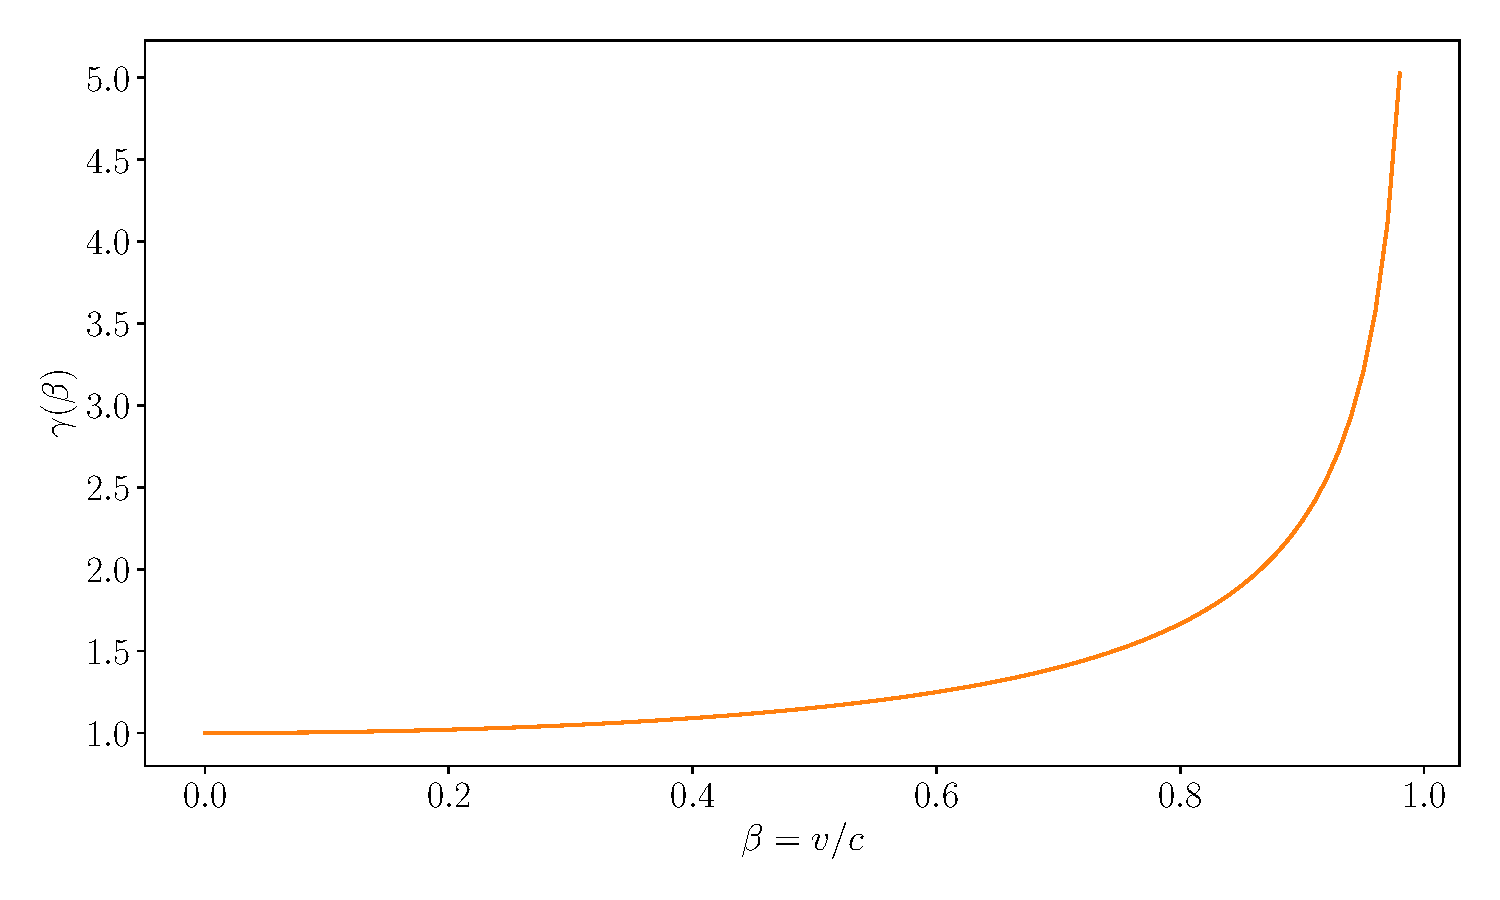
\includegraphics[width=0.9\textwidth]{pictures/gamma_factor.pdf}
	
	\caption[Plot of the Lorentz-factor]{Plot of the Lorentz-factor $\gamma = \frac{1}{\sqrt{1 - v^2 / c^2}}$.	Clearly, its effect only becomes significant for speeds which are significant fractions of $c$.}
	\label{fig:gamma_factor}
\end{figure}



\begin{figure}
	\centering

%	\begin{minipage}{0.5\textwidth}
%		\centering

		\begin{tikzpicture}
			\spacetimediagram[onlypositive=true, lightcone=false]{4}
	
			\draw[thick, red, cm={1, 0, 1/2, 1, (0,0)}] (0, 0) rectangle (2, 4);  % "World line" of rod
			\draw[thick, red, dashed, cm={1, 0, 1/2, 1, (0,0)}] (1, 0) -- (1, 4);  % World line of midpoint -> yes, for condition of simultaneity
	
			\draw[thick, lightyellow] (0, 0) -- (2, 2);
			\draw[thick, lightyellow] (0, 4) -- (8/3, 4/3);
	
			\draw[->, thick, blue] (0, 0) -- (4, 2) node[right] {$x'$};
			\draw[->, thick, blue] (2, 4) -- (2.5, 5) node[above] {$ct'$};
	
		\end{tikzpicture}
%	\end{minipage}%
	%
%	\begin{minipage}{0.5\textwidth}
		%\centering

		\caption[Spacetime diagram for a moving rod]{Spacetime diagram for a rod moving with velocity $v$, whose ends are depicted as red lines (midpoint using dashed line).\\
		By definition, the axis $ct'$ is the left end of the rod at $x' = 0$. In the $(ct, x)$-frame, it is given by the line $x = vt$. For the $x'$-axis, one can construct the point on the world line of the right end of the rod that is simultaneous to $t' = 0$ as measured by the left end of the rod. In accordance with the Einstein synchronization, this can be done by looking at light sent out from the origin and its intersection with the midpoint (dashed line). Tracing back this intersection point using light that is sent out by the right end of the rod in negative $x$-direction, one finds the point simultaneous to $t = 0 = t'$ in the origin (i.e.~the line of simultaneity, which is nothing but $x'$).}
		\label{fig:moving_rod_diagram}
%	\end{minipage}
\end{figure}





\iffalse
{ % Too complicated
To obtain the way $t \rightarrow t'$ transforms, we have to think a bit more and in fact, reinterpret the ansatz \eqref{eq:lorentz_spatial_ansatz}. 
-> this is the same as arguing in terms of equilocality for moving measuring rod; if we do this for time, i.e.~think about simultaneity, we end up with ...

Demanding the same structure for $t' \rightarrow t$ means


from that we get $\gamma$


\begin{figure}
	\centering
	
	\begin{tikzpicture}
		\spacetimediagram[onlypositive=true, lightcone=false]{4}

		\draw[thick, red, cm={1, 0, 1/2, 1, (0,0)}] (0, 0) rectangle (2, 4);  % "World line" of rod
		\draw[thick, red, dashed, cm={1, 0, 1/2, 1, (0,0)}] (1, 0) -- (1, 4);  % World line of midpoint -> yes, for condition of simultaneity

		\draw[thick, lightyellow] (0, 0) -- (2, 2);
		\draw[thick, lightyellow] (0, 4) -- (8/3, 4/3);

		\draw[->, thick, blue] (0, 0) -- (4, 2) node[right] {$x'$};
		\draw[->, thick, blue] (2, 4) -- (2.5, 5) node[above] {$ct'$};

	\end{tikzpicture}
	
	\caption{}
\end{figure}


In $x$-coordinates, the point $x' = 0$ moves away at speed $x = vt$


the axis $x'$ is determined from the fact that it consists of all events happening at $t' = 0$, i.e.~those which are simultaneous to origin $(ct', x') = (0, 0)$; we have determined this axis by constructing event $E$ that right end of rod perceives to be simultaneous to $t' = 0$ measured by left end of rod (which crosses origin)

rod does not move in primed coordinates, i.e.~$x' = const$ for it; therefore, by prolonging world line of left end of rod, we get axis where $x' = 0$ for all times $t'$ and thus the axis $ct'$


$\gamma$ is stretching, needed because we know that lengths are measured differently in moving systems

}
\fi



		\subsection{Time Dilation \& Length Contraction 2}\label{subsec:time_dilation_lorentz}
In principle, it is not surprising that a new transformation has to be used. After all, we have demanded some new postulates to be true and there is no reason for the \enquote{old} transformation to fulfil it. On the other hand, we have already examined quite a few predictions of these postulates in the clock section \ref{sec:clocks} and likewise, it is not guaranteed that our new Lorentz transformation reproduces the results which have been found there.

Most prominently, time dilation and length contraction showed up as new effects. We will now check if they can be reproduced in coordinates related via the Lorentz transformation.



			\paragraph{Measuring in Unprimed Coordinates}
Consider a rod with ends at positions $x_1, x_2$. Their spatial distance and thus the length of the rod in unprimed coordinates is
\begin{equation*}
	L = x_2 - x_1 \, .
\end{equation*}

From the primed coordinates, however, one would measure
\begin{equation}\label{eq:length_contraction_not_correct}
	L' = x'_2 - x'_1 = \gamma (x_2 - v t_2) - \gamma (x_1 - v t_1) = \gamma (x_2 - x_1) = \gamma L = \frac{L}{\sqrt{1 - \frac{v^2}{x^2}}} \, .
\end{equation}
Here we assume $t_1 = t_2$ because by definition, distances are measured at the same time (simultaneously). This result is not what we expect from the previous discussions. Is the Lorentz transformation at fault? Luckily, no. We have emphasized how simultaneity is important for the length to be meaningful. However,
\begin{equation}\label{eq:not_simultaneous}
	t'_1 = \gamma (t_1 - \frac{v}{c^2} x_1) \neq \gamma (t_2 - \frac{v}{c^2} x_2) = t'_2
	\quad \Leftrightarrow \quad
	\Delta t' = t'_2 - t'_1 = \gamma \frac{v}{c^2} (x_1 - x_2) \neq 0
	\, ,
\end{equation}
the measurements in primed coordinates are not simultaneous, so this $L'$ is \emph{not} what a ruler in primed coordinates measures. In order to simulate this result, we have to tune the times $t_1, t_2$ to achieve $t'_1 = t'_2$. Choosing
\begin{equation}
	\Delta t = t_2 - t_1 = - \Delta t' = - \gamma \frac{v}{c^2} (x_1 - x_2) = \frac{v}{c^2} \gamma L
\end{equation}
leads to a cancellation of the time difference in \eqref{eq:not_simultaneous}. The \enquote{true} length measured in unprimed coordinates then becomes
\begin{equation}\label{eq:length_contraction_correct}
	\begin{split}
	\eqbox{L'} &= x'_2 - x'_1 = \gamma (x_2 - v t_2) - \gamma (x_1 - v t_1) = \gamma L - v \Delta t
	\\
	&= \gamma L - \frac{v^2}{c^2} \gamma L = \frac{1 - \frac{v^2}{c^2}}{\sqrt{1 - \frac{v^2}{c^2}}} L = \sqrt{1 - \frac{v^2}{c^2}} L = \eqbox{\frac{L}{\gamma}} \, .
	\end{split}
\end{equation}
Moving rulers measure smaller distances, physics is still intact.
Effectively, this corresponds to waiting a longer time until the second measurement in unprimed coordinates, which in turn causes the transformed times $t'_1, t'_2$ to be equal (note that the length $L$ does not change because it is at rest in unprimed coordinates, i.e.~$x_1, x_2$ are constant, independent of time). An intuitive explanation for this is that the moving observer claims the system at rest is moving, i.e.~the end of the rod moves away from him, shortening it. In order to compensate for that, we have to wait a bit longer until taking the second measurement at $t'_2$ and correspondingly, increase $t_2$.\\


Consider a temporal distances $T = t_2 - t_1$ measured by a clock resting in unprimed coordinates (i.e.~$x_1 = x_2$). This time difference measured from primed coordinates is
\begin{equation*}
	%T = t_2 - t_1
	%\qquad \qquad
	T' = t'_2 - t'_1 = \gamma (t_2 - \frac{v}{c^2} x_2) - \gamma (t_1 - \frac{v}{c^2} x_1) = \gamma (t_2 - t_1) = \gamma T = \frac{T}{\sqrt{1 - \frac{v^2}{c^2}}} \, .
\end{equation*}
The primed observer measures a time $T'$ between two events on his clock, while on the clock resting in unprimed coordinates,
\begin{equation}
	\eqbox{
	T = \sqrt{1 - v^2 / c^2} \, T'
	}
\end{equation}
go by. Since the primed observer sees the unprimed one moving, that confirms what we already knew: moving clocks tick slower. This effect can be attributed to the synchronization of clocks. Despite $x_1 = x_2$, $x'_1 \neq x'_2$, so the measurements in primed coordinates are taken by two different clocks (which are properly synchronized, but in the primed frame).



			\paragraph{Measuring in Primed Coordinates}
Now consider a rod with end points at $x'_1, x'_2$. Its length measured from the primed coordinates is
\begin{equation*}\label{eq:rod_primed_coords_from_primed}
	L' = x'_2 - x'_1 \, .
\end{equation*}

This measurement is conducted simultaneously in primed coordinates, so $t'_1 = t'_2$. From unprimed coordinates, however, we measure at $t_1 = t_2$. For this reason, $L'$ becomes
\begin{equation*}
	L' = x'_2 - x'_1 = \gamma (x_2 - v t_2) - \gamma (x_1 - v t_1) = \gamma (x_2 - x_1) = \gamma L \, .
\end{equation*}
Consequently, the length $L$ of the rod measured in unprimed coordinates is
\begin{equation}
	\eqbox{
	L = \frac{L'}{\gamma}
	} \, ,
\end{equation}
which confirms the mutuality of length contraction.


Next, consider a temporal distance $T' = t'_2 - t'_1$ measured by a clock resting in primed coordinates (i.e.~$x'_1 = x'_2$). Measuring in this difference in unprimed coordinates, where the clock has moved from $x_1$ to $x_2 = x_1 + v T, \; T = t_2 - t_1$ during this time, yields
\begin{equation}
	\eqbox{T'} = t'_2 - t'_1 = \gamma (t_2 - \frac{v}{c^2} x_2) - \gamma (t_1 - \frac{v}{c^2} x_1) = \gamma (t_2 - t_1 - \frac{v^2}{c^2} T) \eqbox{= \frac{T}{\gamma}} \, .
\end{equation}
Hence, we have also obtained the mutuality of time dilation.\\


Albeit the calculations are largely equivalent, we have argued slightly differently here, which was done deliberately to show there is not a single correct way of calculating the corresponding effects. In the end, we can can confirm that both length contraction and time dilation are reproduced by the Lorentz transformation. Furthermore, the calculations are much more straightforward compared to what had to be done previously (setting up synchronization, drawing complicated diagrams etc.). For this reason, it is customary to introduce the Lorentz transformation without covering any details on clocks. However, in my personal experience, that often results in a lack of intuition on these topics -- one is bound to the understanding in terms of Lorentz transformations, although they are \emph{not} necessary to understand what is going on. Since special relativity is a confusing topic in itself due to several frames and new concepts, intuition is an important part and helps tremendously with interpreting calculations.



		\subsection{Addition of Velocities}
Let us now turn to velocities in relativity. Intuitively, we expect the velocity of points with fixed coordinates in the primed frame to move with velocity $v$ in the unprimed frame, i.e.~we expect them to fulfil an equation of the form
\begin{equation*}
	x = v t + b
\end{equation*}
for some offset/shift $b$. However, looking at the Lorentz transformation \eqref{eq:lorentz_trafo}, we may get confused by all the $\gamma$'s and ask ourselves: is this really the case? Rearranging yields
\begin{equation}
	x = v t + x' / \gamma
\end{equation}
as the world line of a fixed point $x'$ in unprimed coordinates $(x, c t)$. Hence, the velocity of this world line (again, in unprimed coordinates) is
\begin{equation}
	\dv{x}{t} = \dv{t} (v t + x' / \gamma) = v \, .
\end{equation}
Velocities work as expected between two uniformly moving frames.\\


As more frames get involved, something has to be different though. This is because of $c$ being a universal speed limit, so adding velocities in relativity cannot work as before, which would allow velocities $> c$. To find out how it works, let us look at a third frame $(x'', c t'')$ moving with velocity $w$ relative to $(x', c t')$. Inserting the Lorentz transformation twice yields
\begin{align*}
%	x'' &= \gamma_w \qty(x' - w t') = \gamma_w \qty(\gamma_v (x - v t) - w \gamma_v \qty(t - \frac{v}{c^2} x))
%	\notag\\
%	&= \frac{1}{\sqrt{1 - w^2 / c^2}} \frac{1}{\sqrt{1 - v^2 / c^2}} \qty(x + \frac{v w}{c^2} x - (v + w) t)
%	\notag\\
%	&= \frac{1}{\sqrt{(1 + w^2 / c^2) (1 - v^2 / c^2)}} \qty(\qty(1 - \frac{v w}{c^2}) x - (v + w) t)
%	\notag\\
%	&= \frac{1}{\sqrt{1 - (v^2 + w^2 + (v w)^2) / c^2}} \qty(\qty(1 + \frac{v w}{c^2}) x - (v + w) t)
%
% Writing out gamma factors not needed, is it?
	x'' &= \gamma_w \qty(x' - w t') = \gamma_w \qty(\gamma_v (x - v t) - w \gamma_v \qty(t - \frac{v}{c^2} x))
	\notag\\
	&= \gamma_v \gamma_w \qty(\qty(1 - \frac{v w}{c^2}) x - (v + w) t)
\end{align*}
Thus, the world line of $x'' = 0$ (convenient choice, no offset, so that velocity can be read off immediately) is given in the unprimed $(x, ct)$-coordinates by
\begin{equation}\label{eq:velocity_addition_parallel}
	x'' = 0
	\qquad \Leftrightarrow \qquad
	x = \frac{v + w}{1 + v w / c^2} \, t
	\qquad \Leftrightarrow \qquad
	\eqbox{
	v +_R w = \frac{v + w}{1 + v w / c^2}
	} \, .
\end{equation}
Relativistic addition of velocities is much more complicated than non-relativistic. But setting $v = c$ we see that
\begin{equation}
	\eqbox{
	c +_R w = \frac{c + w}{1 + c w / c^2} = c \frac{1 + w / c}{1 + w / c} = c
	} \, ,
\end{equation}
the $+_R$ we have derived does admit the correct behaviour. Moreover, for $v, w \ll c$
\begin{equation}\label{eq:velocity_addition_limit}
	v +_R w = \frac{v + w}{1 + v w / c^2} \approx v + w \, ,
\end{equation}
it reduces to the usual addition in the Newtonian limit. Thus, we have to accept that addition now works differently, $+_R$ conforms everything we demand from it.\\


Until now, we have assumed $v, w$ to be parallel because we have only taken into account a single spatial dimension. In the more general case with three spatial dimensions, however,
\begin{equation}
	\eqbox{
	\vec{v} +_R \vec{w} \neq \vec{w} +_R \vec{v}
	} \; \text{ and } \;
	\eqbox{
	\vec{v}_1 +_R (\vec{v}_2 +_R \vec{v}_3) \neq (\vec{v}_1 +_R \vec{v}_2) +_R \vec{v}_3
	} \, ,
\end{equation}
adding velocities relativistically is neither commutative nor associative.


% Write out expressions from Giulini (2.6)?





		\subsection{Spacetime Diagrams 2}
Even more help with understanding relativity is provided by visualizations like spacetime diagrams, which are especially helpful because one can visualize multiple observers in a single diagram (see e.g.~fig.~\ref{fig:moving_rod_diagram} or fig.~\ref{fig:spacetime_diagram_two_observers}, where grid lines are shown as well). Essentially, this is a geometric way of visualizing what Lorentz transformations do. By marking the coordinates $(x, ct)$ of an event in a single, resting frame we can immediately read off the coordinates in other frames as well by showing the axes as it is done in \ref{fig:spacetime_diagram_two_observers}. In principle, a Lorentz transformation shifts the points $(x, ct) = (0, ct)$ by $-vt$ to the left. This means the $ct'$-axis is rotated to the left compared to the $ct$-axis, so events would have different positions in diagrams. For this reason, the $ct'$-axis is rotated to the right, such that the position of events stays the same (an analogous argument can be made for the $x'$-axis). Reading off coordinates then works by looking at the transformed lines of simultaneity (parallel to $x'$-axis) and equilocality (parallel to $ct'$-axis), i.e.~projecting the event parallel to these lines until we find the intersection with the $ct'$- and $x$-axis, respectively.


%explanation why primed axes are shifted inwards in Minkowski diagrams: we wish to express these axes in the unprimed coordinate system, i.e.~we do not apply the Lorentz transform from unprimed (at rest) to primed (moving with $v$), but rather the inverse one (thus we have to use $-v$ in transformation) -> better explanation: we wish to draw only one point for events; since a coordinate change from unprimed to primed would rotate the $ct$-axis (where $x = 0$) by $-vt$ and thus to the left ($ct'$ would then by $y$-axis), we have to rotate the $ct'$-axis by the same amount to the right; then, we can read off coordinates of an event in the unprimed and primed frame at once


We have already discussed the causal structure of relativity, timelike trajectories are always in the light cone and spacelike ones are outside of it. For this reason, the events marked by red dots in figure \ref{fig:spacetime_diagram_spacelike} are clearly spacelike. Now we get a a visual explanation of why spacelike events are problematic: while the unprimed, resting observer sees the left event $E_1$ happening before the right one $E_2$, the primed observer sees $E_2$ happening before $E_1$. Thus, if $c$ was not the speed limit and spacelike events were able to communicate with each other, observers could disagree on cause and effect. Luckily, no evidence for such a transmission with $v > c$ has been found (yet), so we do not have to rebuild our understanding of causality.\\



\begin{figure}
	\centering
	
	\begin{tikzpicture}[scale=1.2]
		% Declare numbers as tikz variables, makes changing very convenient
		\tikzmath{\v = 0.5;}

		% Add basis for diagram
		\spacetimediagram{4}
	
		% Add other observer (one sufficient, for more diagram gets increasingly confusing)
		\addobserver{3}{\v}
	
		%\lightcone{1}{-1}{1}{2}
	
		% Add event in rest frame
		\addevent{0}{2}
		\addevent{2}{2}
	
		% Add same event in moving frame
		\addevent[v=\v, color=blue]{0}{2}
		\addevent[v=\v, color=blue]{2}{2}
	\end{tikzpicture}
	
	\caption[Events in frames moving with $v = 0.5 c$ relative to each other]{Events in frames moving with $v = 0.5 c$ relative to each other. Red dots show two events at spacetime points $(x, ct) = (0,2), (2,2)$ (the corresponding primed coordinates are $(x', ct') = (-1.15, 2.3), (1.15, 1.15)$). Blue dots show the same coordinates in the $(x', ct')$-frame (corresponding unprimed coordinates: $(x, ct) = (1.15, 2.3), (3.46, 3.46)$).\\
	We can see very nicely how each observer perceives time differently. Events happening simultaneously to both red dots (i.e.~which lie on the line between them at $t = 2$), do \emph{not} happen at $t' = t$, but at $t' = \tau = \sqrt{1 - v^2} \, t$ (which is evident from the fact that the blue dots are at $t' = t$). The same can be said for the moving observer in blue, which sees events at $t = \sqrt{1 - v^2} \, t'$ simultaneous to the blue dots at $t' = 2$. Analogous arguments can be made for positions and equilocality.}
	\label{fig:spacetime_diagram_two_observers}
\end{figure}



\begin{figure}
	\centering
	
	\begin{tikzpicture}[scale=1.2]
		% Declare numbers as tikz variables, makes changing very convenient
		\tikzmath{\v = 0.5;
				  \Eonex = -1; \Eoney = 2;
				  \Etwox = 2.5; \Etwoy = 3; % For spacelike, velocity times x-coordinate difference has to be greater than time-coordinate difference
				 }

		% Add basis for diagram
		\spacetimediagram[lightcone=false]{4}
	
		% Add other observer (one sufficient, for more diagram gets increasingly confusing)
		\addobserver{3}{\v}
	
	
		% Add event in rest frame
		\lightcone[xpos=\Eonex, ypos=\Eoney]{2}
		\addevent[label=$E_1$]{\Eonex}{\Eoney}
		\addevent[label=$E_2$]{\Etwox}{\Etwoy}
	\end{tikzpicture}
	
	\caption[Spacelike events]{Spacelike events.\\
	It is very obvious that $E_2$ does not lie in the light cone of $E_1$, which has been visualized to make that clear (this implies $E_1$ does not lie in the light cone of $E_2$). The unprimed, black observer sees $E_1$ happening before $E_2$, while the blue observer moving at $v = 0.5 c$ sees it the other way around.}
	\label{fig:spacetime_diagram_spacelike}
\end{figure}



The new addition of being able to depict multiple observers to spacetime diagrams makes them a powerful tool suitable to explain many effects of relativity. For example, the fairly complicated twin paradox can be explained and -- perhaps, even more important -- visualized conveniently.

\begin{ex}[Twin Paradox 2]\label{ex:twin_paradox_2}
	As promised, here comes the detailed demonstration of the twin paradox, which has been started in example \ref{ex:twin_paradox_1}. We will discuss the setup shown in figure \ref{fig:twin_paradox}, i.e.~treat one observer at rest (will be commonly referred to as \enquote{unprimed} one) and two observers moving with velocities $v = \pm 0.5 c$ relative to the unprimed observer (these will be called \enquote{primed} and \enquote{double-primed}, in accordance with their axis labels in \ref{fig:twin_paradox}).
	
	Our approach will be to compute the roundtrip time needed to go from $S$ to $E$ (i.e.~the time passing on the world line on $ct$ axis) and the time needed to go from $S$ to $T$ to $E$ (i.e.~the time passing on the other world line shown in \ref{fig:twin_paradox}). Each of these quantities will be computed from clocks resting in all three of the inertial frames shown in figure \ref{fig:twin_paradox} (reminder: three are involved due to turning around, rest frame of moving observer changes there).\\
	
	%the thing that makes things make sense is that all observers agree on the time passing along moving clock, even when measured from their coordinates; after all, from the double-primed coordinates we can still look at time passing on clock in primed coordinates and simultaneously passing in rest frame; adding that up, we get the total times and these agree between the frames (good, otherwise we would have problem)
	
	During the process, we have to distinguish between four times: (i) the time $t_{ST}$ passing on the resting clock between $S$ and $T$, (ii) the time $t_{TE}$ passing on the resting clock between $T$ and $E$, (iii) the time $\tau_{ST}$ passing on the moving clock between $S$ and $T$ and (iv) the time $\tau_{TE}$ passing on the moving clock between $T$ and $E$. From that we get the total times for resting and moving clock,
	\begin{equation*}
		t_{SE} = t_{ST} + t_{TE}
		\manyqquad
		\tau_{SE} = \tau_{ST} + \tau_{TE} = t'_{ST} + t''_{TE} \, .
	\end{equation*}
	
	One final note concerns the velocities involved: the world line is drawn for $v = 0.5 c$ on the way from $S$ to $T$ and $v = -0.5 c$ on the way from $T$ to $E$ (same velocity, different direction), where $v$ is the velocity of the respective moving frame compared to the unprimed, resting one. This implies a relative velocity of
	\begin{equation*}
		v_2 = \frac{0.5 c + 0.5 c}{1 + 0.5^2} = 0.8 c
	\end{equation*}
	from double-primed to primed frame.
	
	\begin{itemize}
		\item \textbf{Measuring from unprimed coordinates}
		
		Clearly,
		\begin{equation*}
			t_{ST} = 2 = t_{TE}
			\qquad \Leftrightarrow \qquad
			t_{SE} = t_{ST} + t_{TE} = 4
		\end{equation*}
		in arbitrary time units (where one time unit goes by between two grid lines). From that, Minkowski's theorem tells us
		\begin{equation*}
			t'_{SE} = \sqrt{1 - v^2} \, t_{SE} = 3.464 \, .
		\end{equation*}
	
		Simultaneously, by looking at how much time elapses between the intersection of gray grid lines and the blue $ct'$-axis, one can see that as a rough estimate $t'_{ST} \lesssim 2$. For the exact result, we apply Minkowski's theorem:
		\begin{equation*}
			t'_{ST} = \tau_{ST} = \sqrt{1 - v^2 / c^2} \, t_{ST} = \sqrt{1 - 0.5^2} \cdot 2 = 1.732 \, .
		\end{equation*}
		Applying the same procedure to the double-primed coordinates yields
		\begin{equation*}
			t''_{TE} = \tau_{TE} = \sqrt{1 - v^2 / c^2} \, t_{TE} = \sqrt{1 - (-0.5)^2} \cdot 2 = 1.732 = \tau_{ST} \, .
		\end{equation*}
		
		This is because time dilation does not depend on the direction, only on the absolute velocity. Therefore, we can confirm that
		\begin{equation*}
			t_{SE} = t_{ST} + t_{TE} = 4 > \tau_{SE} = \tau_{ST} + \tau_{TE} = 3.464 \, ,
		\end{equation*}
		less time goes by on the moving clock.\\
		
	
	
		\item \textbf{Measuring from primed coordinates}
	
		While from these coordinates one still sees four time units going by on the roundtrip for the resting observer, i.e.~$t_{SE} = 4$, a rough estimate for the roundtrip time measured by a clock resting in the primed coordinates $ct'$ is $t'_{SE} \gtrsim 4$. More precisely, Minkowski's theorem yields
		\begin{equation*}
			t_{SE} = \sqrt{1 - v^2 / c^2} \, t'_{SE}
			\qquad \Leftrightarrow \qquad
			t'_{SE} = \frac{t_{SE}}{\sqrt{1 - v^2 / c^2}} = \frac{4}{\sqrt{1 - (-0.5)^2}} = 4.619 \, .
		\end{equation*}
		This is a consequence from the mutuality of time dilation, an observer resting in primed coordinates sees the unprimed observer moving at $v = -0.5 c$ and therefore measures more time passing in his own frame.
	
	
		However, $t'_{SE}$ is not what a clock in the primed coordinates sees. Instead, 
		\begin{equation*}
			\tau_{SE} = \tau_{ST} + \tau_{TE} = t'_{ST} + t''_{TE}
		\end{equation*}
		as stated before. For $t'_{ST}$, however, we cannot simply use Minkowski's theorem and thus the time
		\begin{equation*}
			\frac{t_{ST}}{\sqrt{1 - v^2 / c^2}} = 2.309 \, ,
		\end{equation*}
		which cannot be quite correct since from the diagram we get the estimate $t'_{ST} \lesssim 3$. This is because the world line is moving with respect to the rest frame of $ct$, so we would only get statements about what is the time as seen from this frame. However, we wish to measure the primed time from the primed coordinates. This requires a Lorentz transformation of the events $S, T, E$:
		\begin{equation*}
			t'_{ST} = t'_T - t'_S = \frac{t_T - \frac{v}{c} x_T}{\sqrt{1 - v^2 / c^2}} - \frac{t_S - \frac{v}{c} x_S}{\sqrt{1 - v^2 / c^2}} = \frac{t_{ST} - \frac{v}{c} x_T}{\sqrt{1 - v^2 / c^2}} = \frac{2 - 0.5 \cdot 1}{\sqrt{1 - 0.5^2}} = 1.732 \, .
		\end{equation*}
		In the same manner, we obtain
		\begin{equation*}
			t'_{TE} = t'_E - t'_T = \frac{t_E - \frac{v}{c} x_E}{\sqrt{1 - v^2 / c^2}} - \frac{t_T - \frac{v}{c} x_T}{\sqrt{1 - v^2 / c^2}} = \frac{t_{TE} + \frac{v}{c} x_T}{\sqrt{1 - v^2 / c^2}} = \frac{2 + 0.5 \cdot 1}{\sqrt{1 - (-0.5)^2}} = 2.887 \, .
		\end{equation*}
	
		To get $t''_{TE}$, we have to prolong the axes of simultaneity of the primed coordinates and count the number of time units which go by between the intersections of them with $ct''$ (i.e.~the number of intersections with green lines on the way). This yields roughly $t''_{TE} \gtrsim 1.5$ again. For the time passing simultaneously on a clock in primed coordinates, we can read off roughly $t'_{TE} \approx 4$. The correct numbers can be obtained from Minkowski's theorem again:
		\begin{equation*}
			t''_{TE} = \sqrt{1 - (-v_2)^2 / c^2} \, t'_{TE} = \sqrt{1 - (-0.8)^2} \, 2.887 = 1.732 \, .
		\end{equation*}
	
		All together, the primed observer measures a roundtrip time
		\begin{equation*}
			t'_{SE} = t'_{ST} + t'_{TE} = 4.619 > \tau_{SE} = \tau_{ST} + \tau_{TE} = t'_{ST} + t''_{TE} = 3.464 \, .
		\end{equation*}
		We find the same result that less time has passed on the moving clock. Furthermore, we see that the absolute value for this $\tau_{SE} = t'_{SE}$ and the one computed from Minkowski's theorem in the first calculation agree (because corresponding world line is parallel to $ct$). On the other hand, it should not be surprising that the absolute values measured for $\tau_{ST}$ and $\tau_{TE}$ do not agree. After all, they are still measured from different reference frames and with respect to frames moving with different relative velocities ($\pm 0.5$ for primed; $0.5, 0.8$ for unprimed).\\
	
		
		% for v=0.7 c
		%on own clock, six time units go by for roundtrip; however, he agrees that just four go by on resting clock
		
		%on own clock, it is again roughly $3 / 2$ which pass by; on $ct''$ he sees $3 / 2$ passing by as well (way to see that: look at which lines parallel to $x'$ intersect the relevant events, i.e.~starting point and turning point; then look at points where these lines intersect $ct''$ and count number of ticks on $ct''$ between these intersections); in the same manner, we see that four time units pass on $ct$
		
		\item \textbf{Measuring from double-primed coordinates}
	
		Just as before, $t_{SE} = 4$ is measured, while roughly $t''_{SE} \gtrsim 4$ and precisely
		\begin{equation*}
			t''_{SE} = \frac{t_{SE}}{\sqrt{1 - v^2 / c^2}} = \frac{4}{\sqrt{1 - (-0.5)^2}} = 4.619
		\end{equation*}
		are measured by a clock resting in the double-primed coordinates. As one can confirm by looking at the result above, this is the same time a clock resting in primed coordinates measures. We expect more of these equal results since the double-primed coordinate system is moves with the same relative velocity as the primed one, just in the other direction (sign of velocity is different).
	
		A rough estimate for $t''_{TE}$ is $t''_{TE} \gtrsim 2$ and the exact result is
		\begin{equation*}
			t''_{TE} = t''_E - t''_T = \frac{t_E - \frac{v}{c} x_E}{\sqrt{1 - v^2 / c^2}} - \frac{t_T - \frac{v}{c} x_T}{\sqrt{1 - v^2 / c^2}} = \frac{t_{TE} + \frac{v}{c} x_T}{\sqrt{1 - v^2 / c^2}} = \frac{2 - 0.5 \cdot 1}{\sqrt{1 - (-0.5)^2}} = 1.732 \, .
		\end{equation*}
		An analogous calculation yields
		\begin{equation*}
			t''_{ST} = t''_T - t''_S = \frac{t_T - \frac{v}{c} x_T}{\sqrt{1 - v^2 / c^2}} - \frac{t_S - \frac{v}{c} x_S}{\sqrt{1 - v^2 / c^2}} = \frac{t_{ST} - \frac{v}{c} x_T}{\sqrt{1 - v^2 / c^2}} = \frac{2 + 0.5 \cdot 1}{\sqrt{1 - 0.5^2}} = 2.887 \, .
		\end{equation*}
		As promised, we get more results that we have already seen in calculations in the primed coordinates, but now they are switched (due to the transition $v \rightarrow -v$).
	
		Now we wish to compute $t'_{ST}$ and expect roughly $t'_{ST} \gtrsim 1.5$. Indeed, we obtain
		\begin{equation*}
			t'_{ST} = \sqrt{1 - v_2^2 / c^2} \, t'_{TE} = \sqrt{1 - 0.8^2} \, 2.887 = 1.732 \, .
		\end{equation*}
		All in all, the double-primed observer measures a roundtrip time
		\begin{equation*}
			t''_{SE} = t''_{ST} + t''_{TE} = 4.619 > \tau_{SE} = \tau_{ST} + \tau_{TE} = t'_{ST} + t''_{TE} = 3.464 \, .
		\end{equation*}
		Once again, these results look very familiar. 
	\end{itemize}
	
	
	
	A conclusion of these extensive calculations is that physics is not broken, despite relativity sometimes being unintuitive at first glance. All inertial frames play equal roles, which shows in the mutual slowing of moving clocks. In frames where both clocks seem to be moving, we can further confirm that the effect increases with the velocity $v$, as implied by \eqref{eq:minkowski_theorem}.
	
	It should also be noted that the agreement of all three observers regarding $\tau_{SE}$ is really a coincidence due to the symmetric setup we have chosen -- for other scenarios, e.g.~with unequal velocities on the first and second part of the journey or even if we assume that $ct$ is not at rest after all (but keeping the relative velocities of primed and unprimed system, i.e.~rotating the whole setup), this will not be the case anymore. In the same manner,
	\begin{equation*}
		t'_{ST} \neq t''_{TE}
	\end{equation*}
	in general. However, if one of the clocks moves on a world line parallel to the $ct$-axis of one of the observers, \emph{all} of them will agree on the time elapsed along this clock (so $t_{SE}$ being equal for all observers is really not a coincidence; the same goes for $t'_{ST}$ and $t''_{TE}$ in this setup). This is despite observers measuring different times on their own clocks and is due to Minkowski's theorem, which tells us how much time has passed simultaneously on a clock in another frame.


-> note: although there is no preferred system in the sense that it is \enquote{more correct} than others (no absolute space), one can argue it numbers computed in stationary system are the ones that make most sense because assuming the moving observer stops again and rests after his journey, this rest frame is where they compare their clocks in and thus also where an experiment would be conducted (i.e.~these times would be the one which are measured)
\end{ex}



\begin{figure}
	\centering

	\begin{tikzpicture}[scale=1.2]
		% Declare numbers as tikz variables, makes changing very convenient
		\tikzmath{\vprime = 0.5; \vdoubleprime = -0.5;
				  \tS = -2; \tT = 0;
				  \tE = 2; \xS = 0;
				  \xT = (\tT - \tS) * \vprime; \xE = 0;
				  }  % Note: world line connecting S and T is always parallel to time axis of primed observer, while world line connecting T and E is only parallel to double-primed if vprime=-vdoubleprime

		% Add basis for diagram
		\spacetimediagram{4}
	
		% Add other observers
		\addobserver{3}{\vprime}
		\addobserver[xlabel=$x''$, ylabel=$ct''$, color=black!40!green]{3}{\vdoubleprime}

		% Add worldlines of clocks and start, end events
		\addworldline{\xS}{\tS}{\xT}{\tT}  % Resting clock
		\addworldline{\xS}{\tS}{\xT}{\tT}  % Moving clock
		\addworldline{\xT}{\tT}{\xE}{\tE}  % Moving clock

		\addevent[radius=2pt, label=$S$, label placement=right]{\xS}{\tS}  % S
		\addevent[radius=2pt, label=$T$, label placement=right]{\xT}{\tT}  % T
		\addevent[radius=2pt, label=$E$, label placement=right]{\xE}{\tE}  % E
	\end{tikzpicture}

	\caption[Visual explanation of twin paradox]{Visual explanation of twin paradox. Event $S$ is the starting point, $T$ turning point and $E$ end point. The primed observer has a relative velocity of $v = 0.5 v$ with respect to the unprimed one, while the double-primed observer has $v = -0.5 c$.\\
	We can measure times passing between events in a certain frame $\mathcal{O}$ by prolonging the corresponding lines of simultaneity (parallel to spatial axis of $\mathcal{O}$) from event to the time axis of $\mathcal{O}$ and then count the number of time units passing on the time axis between the intersection points. Similarly, we could also prolong them until they intersect the time axis of any other frame $\mathcal{O}'$. In this case, counting the number of time steps passing between the intersection points on the time axis of $\mathcal{O}'$ would yield the time passing for $\mathcal{O}'$, measured from $\mathcal{O}$.}
	\label{fig:twin_paradox}
\end{figure}






\end{document}